% options:
% thesis=B bachelor's thesis
% thesis=M master's thesis
% czech thesis in Czech language
% slovak thesis in Slovak language
% english thesis in English language
% hidelinks remove colour boxes around hyperlinks

\documentclass[thesis=B,czech]{FITthesis}[2012/06/26]

\usepackage[utf8]{inputenc} % LaTeX source encoded as UTF-8

\usepackage{graphicx} %graphics files inclusion
% \usepackage{amsmath} %advanced maths
% \usepackage{amssymb} %additional math symbols

\usepackage{dirtree} %directory tree visualisation
%\usepackage[]{algorithm2e}
\usepackage{algorithm}
\usepackage{algpseudocode}
\usepackage{pifont}


\usepackage{float}

%\usepackage{listings}
%\lstset{frame=lrbt,xleftmargin=\fboxsep,xrightmargin=-\fboxsep, showstringspaces=false}
  

\usepackage{listings}
\newcommand{\liststy}{\small\ttfamily}

% general command to set parameter(s) ... change to suit your needs
\lstset{
  basicstyle=\liststy, % print whole listing small
  keywordstyle=\color{black}\bfseries,
  identifierstyle=, % nothing happens
  commentstyle=\color{white}, % white comments
  stringstyle=\ttfamily, % typewriter type for strings
  showstringspaces=false
  numbers=left, 
  numberstyle=\tiny,
  numberbychapter=true,
  xleftmargin=0\linewidth,
  xrightmargin=0\linewidth,
  boxpos=c,
  frame=TB, 
  numbersep=2p,
  columns=fullflexible,
  escapechar=`
}

% % list of acronyms
% \usepackage[acronym,nonumberlist,toc,numberedsection=autolabel]{glossaries}
% \iflanguage{czech}{\renewcommand*{\acronymname}{Seznam pou{\v z}it{\' y}ch zkratek}}{}
% \makeglossaries

\newcommand{\tg}{\mathop{\mathrm{tg}}} %cesky tangens
\newcommand{\cotg}{\mathop{\mathrm{cotg}}} %cesky cotangens

% % % % % % % % % % % % % % % % % % % % % % % % % % % % % % 
% ODTUD DAL VSE ZMENTE
% % % % % % % % % % % % % % % % % % % % % % % % % % % % % % 

\department{Katedra Softwarového inženýrství}
\title{Webový server pro poskytování dynamicky generovaných objektů ve formátech RDF}
\authorGN{Jan} %(křestní) jméno (jména) autora
\authorFN{Řasa} %příjmení autora
\authorWithDegrees{Jan Řasa} %jméno autora včetně současných akademických titulů
\supervisor{RNDr. Jakub Klímek, Ph.D.}
\acknowledgements{Chtěl bych poděkovat vedoucímu mé práce RNDr. Jakubu Klímkovi za odborné vedení, pomoc při zpracování této práce a cenné rady.
Dále bych chtěl také poděkovat svým rodičům a přátelům za podporu nejen při tvorbě této práce, ale po celou dobu studia.}
\abstractCS{Řada objektů na webu dat tvoří natolik velkou skupinu (až nekonečnou), že je není možné všechny 
perzistentně uložit a publikovat. Je nutné nabídnout server, který na základě požadavku klienta na daný 
objekt příslušná data dynamicky vygeneruje a odešle klientovi.


Tato práce se zabývá analýzou již existujících řešení, návrhem a implementací daného serveru včetně otestování základní funkcionality.
Server bude umožňovat uživateli definovat RDF (Resource Description Framework) entities pro dynamické 
generování v několika formátech.
Návrh bude zohledňovat již zaběhlé technologie z oboru Linked Data, jako je například dotazovací 
jazyk SPARQL (Protocol and RDF Query Language). Server bude implementován v jazyce Java.}

\abstractEN{There are many objects on the web of data that make such a big group (almost infinite) that it's not possible to persist them all and publish them.
It's necessary to offer a web server that to the client's requests to the given objects dynamically generates the data and sends them back to the client.

The goal of this bachelor's thesis is an analysis of existing solutions, to design and implement this web server, including tests of the basic functionality.
Users of the web server will be able to define RDF (Resource Description Framework) entities for dynamically generating in the several formats.
The design will include popular technologies from Linked Data such as SPARQL language  (Protocol and RDF Query Language). The server will be implemented
in Java.
}

\placeForDeclarationOfAuthenticity{V~Praze}
\declarationOfAuthenticityOption{4} %volba Prohlášení (číslo 1-6)
\keywordsCS{sémantický web, web dat, Linked Data, RDF, dynamické generování, SPARQL, Java, webový server \newpage}

\keywordsEN{semantic web, web of data, Linked Data, RDF, dynamically generating, SPARQL, Java, web server}

\begin{document}

% \newacronym{CVUT}{{\v C}VUT}{{\v C}esk{\' e} vysok{\' e} u{\v c}en{\' i} technick{\' e} v Praze}
% \newacronym{FIT}{FIT}{Fakulta informa{\v c}n{\' i}ch technologi{\' i}}

\begin{introduction}
\paragraph{}
Při publikování dat na webu dat je vždy důležité zamyslet se nad tím, jak a kde budou tyto data uložena.
Způsobů je mnoho. Mezi ty nejzákladnější patří ukládání dat do různých databázových systémů, nebo pouze přímo na určené místo na disku.
Oba zmíněné způsoby a jim podobné mají ovšem jeden zásadní problém, a tím je kapacita uložiště.

Pro uložení většiny informací, se kterými se lze setkat na webu, jako jsou obrázky, zprávy, informace o počasí a mnoho dalších, se tato skutečnot nemusí příliš řešit.
Kapacita uložiští nám pro tyto informace většinou stačí. Nicméně existuje řada informací (dále také objektů), které tvoří natolik velkou skupinu (až nekonečnou),
že je není možné všechny perzistentně uložit a publikovat.

Dobrým příkladem jsou například časová data - konkrétní čas či časový interval. V kontextu Linked Data \cite{linked_data} se často odkazuje na časový objekt.
Ať už se jedná například o časy příjezdů autobusů, časy uvedené ve statistických údajích,
nebo o datum nějaké události, vždy je potřeba mít daný časový objekt nějakým způsobem uložen.

Existují ale kapacity na uložení každého takového objektu? Časových objektů je přeci nekonečně mnoho. Mohou odkazovat jak do minulosti, tak do budoucnosti.
A není potřeba se omezovat pouze na časové objekty. Jako další příklad může být informace o vztahu mezi lidmi, respektive mezi kterýmikoliv subjekty.
Tyto informace taktéž vyžadují ohromné kapacity uložiští.

Mnoho typů objektů ale spojuje fakt, že mají vždy stejnou strukturu a jen část informací se mění (například jen sekunda, hodina, \ldots).
A to je ideální příležitost pro to, aby se ukládání těchto objektů zaměnilo za dynamické generování. Pro vygenerování objektu stačí vždy použít stejnou strukturu
a jen dosadit potřebné informace tak, aby vznikl požadovaný objekt.

\end{introduction}

\chapter{Cíl práce}
Cílem této práce je navrhnout, implementovat a otestovat webový server pro poskytování dynamicky generovaných objektů v RDF formátech.
Server bude splňovat následující požadavky:

 \begin{itemize}
  \item Server bude umožňovat administrátorovi založit nový typ objektů včetně jejich atributů a umožní nakonfigurovat URL, pod kterými budou objekty dostupné. 
  \item Typy objektů bude možné založit přes konfigurační soubor. 
  \item Klient bude moci přístupem na dané URL získat data o příslušném objektu. 
  \item Data o objektech budou klientům dostupná v RDF serializacích (RDF/XML, Turtle, N-Triples, JSON-LD) a jako webová stránka.
  \item Server bude využívat mechanismu Content Negotiation pro určení formátu výstupu požadavku klienta. 
  \item Server bude implementován v jazyce Java.
 \end{itemize}
\chapter{Analýza}

Tato kapitola se zabývá analýzou vyvíjené aplikace. Zmíněn je účel aplikace, analýza již existujících řešení a analýza požadavků kladených na tuto aplikaci.
Cílem analýzy je stanovit základní funkce aplikace a zjistit možné konkurující aplikace, analyzovat je a navrhnout vylepšení, které bude později implementováno.

\section{Účel aplikace}
Webový server bude poskytovat uživatelům funkci pro dynamické generování objektů ve formátech RDF.
Uživatel si bude moci nadefinovat vlastní typy objektů pomocí šablony včetně URL, na které budou dané objekty přístupné.
Objekty budou generovány za použití informací, které bude obsahovat URL adresa při požadavku na daný objekt.

Tento způsob generování objektů ve velké míře šetří především finanční zdroje za pořizování nových uložišť. Pro velké množství stejných objektů (až nekonečně mnoho)
stačí vytvořit pouze jednu definici (šablonu) objektu, která se dle specifikovaných pravidel vyplní informacemi z URL adresy a uživateli se zobrazí jako 
požadovaný objekt.

Další výhodou je z hlediska jednotné definice objektů i možnost lehce upravit strukturu konkrétních definic na jednom místě.
Na konkrétní definici objektu může být odkazováno s různými parametry z mnoha jiných objektů a jedinou změnou v definici lze ovlivnit informace i v těchto objektech.
Měnit již dříve vytvořené a uložené konkrétní objekty v takovém počtu by bylo téměř nereálné.

Účelem serveru je také chování, které co nejméně omezuje možné klienty \footnote{Zde se klientem rozumí především aplikace které by k objektům přistupovaly.}.
Server využívá principu Content Negotiation \cite{content_negotiation} a podporuje nejpoužívanější typy RDF serializací, včetně možnosti zobrazit informace 
o objektu v HTML podobě při zobrazení prohlížečem.


\section{Existující řešení}
Pro funkce, které má tento server splňovat, neexistuje v současnosti žádné jiné řešení. Minimálně není možné dohledat 
  žádné veřejné řešení, ani informace o nějakém soukromém řešení, které by sloužilo například pro soukromá data v rámci nějaké společnosti. 
  Nicméně existuje velmi populární řešení jednoho typu objektu - časových intervalů, tzv. British Time Intervals, které je hojně používané,
  převážně pak také v rámci dat, které poskytuje britská vláda.
  
\subsection{British Time Intervals}
Pro popis těchto objektů je asi nejlepší odkázat se na konkrétní definici na webové stránce, ze které jsou tyto intervaly dostupné.\cite{british_ti}
\begin{quote}
 Linked data for every time interval and instant into the past and future, from years down to seconds.
 This is an infinite set of linked data. It includes government years and properly handles the transition to the Gregorian calendar within the UK.
\end{quote}
 Zde je vhodné všimnout si hlavně slov \textit{infinite set}, což přesně charakterizuje typy objektů, kterými se tato práce zabývá.

 \subsubsection{Struktura URL} Pro přístup k jednotlivým generovaným objektům slouží URL adresa, která má vždy předepsanou strukturu. Informace, které jsou dostupné
k tomuto datasetu, obsahují popis těchto struktur a jsou veřejně dostupné na stránkách společnosti Epimorphics \cite{ti_structure}. Takovou URL adresou může být například 
\textit{http://reference.data.gov.uk/doc/government-year/\{year1\}-\{year2\}}, kde po dosazení let míto \textit{year1} a \textit{year2} a přístupem na danou adresu získáme požadovaný 
objekt časového intervalu.

\subsubsection{Generování objektu} Takový objekt je tedy dynamicky vygenerován s použitím parametrů z URL adresy. Konkrétní popis toho, jak jsou tyto objekty interně generovány 
není veřejný, ale je velmi pravděpodobné, že je použit minimálně jeden z následujících způsobů:
\begin{itemize}
  \item Předem připravená RDF šablona (v libovolném formátu - Turtle, RDF/XML, N-TRIPLES \ldots) s placeholdery, do kterých se dosadí parametry z URL adresy.
  \item SPARQL \cite{sparql_w3c}\cite{sparql_bob} dotaz s placeholdery.
 \end{itemize}

 

\section{Požadavky}
Tato kapitola obsahuje výčet funkčních a nefunkčních požadavků, které budou na výslednou aplikaci kladeny.

\subsection{Funkční požadavky}
Funkční požadavky jsou:
 \begin{itemize}
  \item přístup k administraci objektů přes více rozhraní
  \item podpora více formátů pro definice a zobrazení objektů
  \item zobrazení existujících definic objektů
  \item administrace definic objektů  
  \item konfigurace objektů bude možná několika způsoby
  \item vygenerování a zobrazení konkrétních objektů
 \end{itemize}
 
 \subsubsection{Přístup k administraci objektů přes více rozhraní}
 Administrátori bude umožněn přístup k definicím objektů dvěma způsoby:
 \begin{itemize}
    \item přes webové rozhraní
    \item přes API
 \end{itemize}
 Oba tyto způsoby budou poskytovat stejnou funkcionalitu. Webovým rozhraním se myslí jednoduchá aplikace pro administraci objektů z webového prohlížeče.
 API bude sloužit k administraci z jiných potenciálních aplikací.
 
 \subsubsection{Podpora více formátů pro definice a zobrazení objektů}
 Server bude podporovat následující formáty pro definice objektů přes API:
 \begin{itemize}
    \item JSON formát
    \item RDF serializace TURTLE \cite{turtle_example}
 \end{itemize}
 Konkrétní vygenerované objekty budou klientům dostupné v těchto RDF serializacích:
 \begin{itemize}
    \item RDF/XML \cite{rdf_xml}
    \item JSON-LD \cite{rdf_json_ld}
    \item N-TRIPLES \cite{rdf_n_triples}
    \item TURTLE 
 \end{itemize}
 Každá definice objektů bude také umožňovat definovat HTML formát objektu pro zobrazení v prohlížeči.
 
 \subsubsection{Zobrazení existujících definic objektů}
  Ve webové aplikaci budou zobrazeny všechny aktuální definice objektů v tabulce s možností konkrétní definici upravit (tedy také zobrazit definici konkrétního objektu)
  nebo smazat přes tlačítka vedle každé definice.
  
  Přes API bude možné získat definice objektů ve dvou formátech:
  \begin{itemize}
    \item RDF serializace
    \item JSON formát
 \end{itemize}
  Konkrétní formát bude určen principem Content Negotiation. Získat půjde seznam všech definic a také konkrétní definice.
 
 \subsubsection{Administrace definic objektů}
  Administrátorovi bude umožněno přidávat nové definice, měnit a mazat již vytvořené definice. Tyto akce budou umožněny jak z webové aplikace, tak i přes API.
  Dále bude moci administrátor definovat objekt konfiguračním souborem v RDF serializaci TURTLE.
  
  
  \subsubsection{Konfigurace objektů bude možná několika způsoby}  
  \label{sec:object_types}
  Konfigurací objektů se zde myslí možné způsoby jak a z čeho se bude generovat výsledný objekt. Server bude podporovat
  následující způsoby:
  \begin{itemize}
    \item generování ze SPARQL šablony - CONSTRUCT dotaz \cite{sparql_bob}
      \subitem Vstupem bude SPARQL šablona CONSTRUCT dotazu s placeholdery \footnote{Placeholder: část šablony, která jasně identifikuje místo, 
      kam se dosadí parametry z URL adresy.}, za které se dosadí při požadavku na objekt hodnoty z URL adresy
      a provede se příkaz který vygeneruje objekt.
      
     \item generování ze SPARQL šablony - vzdálený CONSTRUCT nebo DESCRIBE dotaz \cite{sparql_bob}
      \subitem Vstupem bude SPARQL šablona jako v prvním případě. Navíc bude možné provést DESCRIBE dotaz. Rozdíl oproti prvnímu případu je v tom, že se 
      dotaz přepošle na zvolenou adresu SPARQL Endpointu \cite{sparql_bob}, zde se provede a klientovy je pak vrácen daný objekt.
      
    \item generování z RDF šablony
     \subitem Vstupem bude RDF šablona podporovaných serializací s placeholdery, za které se dosadí při požadavku na objekt hodnoty z URL adresy. 
     
     \item Proxy objekt
      \subitem Server bude umožňovat roli prostředníka při generování objektů. Požadavek na objekt se přepošle na jiný server a výsledek se přeloží
      klientovi dle požadované serializace. Tento způsob umožňuje generování objektů přes jiné aplikace.
 \end{itemize}
 
 
  
  \subsubsection{Vygenerování a zobrazení konkrétních objektů}  
  Klient bude moci přístupem na konkrétní URL adresu získat data o příslušném objektu. Typ RDF serializace nebo zobrazení HTML stránky se určí přes 
  Content Negotiation.

\subsection{Nefunkční požadavky}
Nefunkční požadavky jsou:
\begin{itemize}
    \item server bude implementován v jazyce Java
    \item celá aplikace bude uložena ve WAR souboru pro zjednodušené nasazení
    \item aplikace bude spustitelná v Javě verze 8
    \item k aplikaci budou přiloženy ukázkové objekty
 \end{itemize}
 
 \chapter{Návrh}
 Tato kapitola se zabývá návrhem výsledné aplikace. První část je věnována použitým technologiím. Poté následuje návrh celkové architektury.
 Převážná část této kapitoly je věnována návrhu konkrétních komponent, jako je například API a administrace definic objektů.
 
 
 \section{Použité technologie}
 Cílem této kapitoly je vymezit technologie, které se v této práci budou vyskytovat. Vzhledem k méně znamým technologiím, jako jsou Linked Data,
 jsou tyto technologie i krátce popsány.
 
 \subsection{Resource Description Framework (RDF)}
 Resource Description Framework je rodina specifikací, která se používá jako metoda pro modelování informací - RDF entit.
 Jedná se o model metadat, které popisují nějaké zdroje.
 
 Příkladem může být obyčejná webová stránka obsahující nějaké informace. Webové stránky se zaměřují především na uživatele.
 Důležité je, aby se uživateli stránky líbily a dbá se tedy hodně na design. Pokud jsou stránky přehledné, pak člověk nemívá problémy pochopit
 dané informace. Nicméně stroj (počítač, program) tyto informace sice zobrazí uživateli, ale samotné informace si interpretovat nedokáže.
 
 RDF model popisuje tedy způsoby, jakými docílit toho, že poskytované informace budou čitelné i pro stroje.
 
 Základní kostrou RDF modelu dat jsou takzvané $trojice$. Tyto trojice se skládají ze subjektu, predikátu a objektu.
 Trojice se může volně přeložit i do podoby, kde subjekt má nějakou vlastnost (predikát) s konkrétní hodnotou (objekt). Tedy všechny trojice, které mají
 stejný subjekt tento subjekt definují.
 
 Každý subjekt je identifikován nejčastěji přes IRI. Bavíme-li se o datech na webu, tak zde může být IRI klasická URL adresa, jak ji známe
 z běžného používání. Co se týče objektu (hodnoty), tak se může jednat o literál (řetězec, číslo apod.), ale hodnotou může být zase IRI nějaké další entity.
 Dokonce i predikát může být RDF entitou s vlastním IRI. Tím, že se objekt skládá z dalších entit, které jsou jednoznačně identifikovány pomocí IRI, získáváme velkou výhodu
 tohoto modelu. Ve výsledku vzniká grafová struktura popisující tyto trojice, což je i pro stroje čitelná struktura.
 
 Samotné RDF popisuje pouze model. Pro uložení RDF entit je zapotřebí informace nějakým způsobem serializovat. V rámci RDF se nejčastěji 
 používají tyto serializace:
 \begin{itemize}
  \item RDF/XML
  \item Turtle
  \item N-Triples
  \item JSON-LD
 \end{itemize}
 
 Pro ukázku je zde příklad ve formátu Turtle, který je převzat z W3C specifikace \cite{turtle_example}.
 \begin{lstlisting}[float=htb,caption={RDF Turtle: W3C Enemies},label=list:spage]
@base <http://example.org/> .
@prefix rdf: <http://www.w3.org/1999/02/22-rdf-syntax-ns#> .
@prefix rdfs: <http://www.w3.org/2000/01/rdf-schema#> .
@prefix foaf: <http://xmlns.com/foaf/0.1/> .
@prefix rel: <http://www.perceive.net/schemas/relationship/> .

<#green-goblin>
    rel:enemyOf <#spiderman> ;
    a foaf:Person ;  # in the context of the Marvel universe
    foaf:name "Green Goblin" .

<#spiderman>
    rel:enemyOf <#green-goblin> ;
    a foaf:Person ;
    foaf:name "Spiderman".
\end{lstlisting}

\texttt{<\#green-goblin>} je zde subjekt identifikovaný IRI \url{http://example.org/\#green-goblin},
\texttt{rel:enemyOf} je predikát - v tomto případě zase objekt identifikovaný IRI \url{http://www.perceive.net/schemas/relationship/enemyOf} a 
 \texttt{<\#spiderman>} je objekt - zase identifikován IRI.
 Tento model dohromady poskytuje informaci, že objekt na dané IRI je nepřítelem Spidermana. \texttt{a foaf:Person} znamená, že
 se jedná o objekt Person a \texttt{foaf:name "Green Goblin"} zase to, že jeho jméno je Green Goblin.
 Tímto je tedy definován objekt \texttt{<\#green-goblin>} a podobně tomu je u 
 objektu \texttt{<\#spiderman>}.
 
 \subsection{Linked Data}
  Linked data, jak už název napovdá, popisuje metodu propojování informací na webu dat mezi sebou.  
  Tim Berners-Lee popisuje Linked Data výstižně takto: 
  \uv{\textit{Semantic Web isn't just about putting data on the web. It is about making links, so that a person or machine can explore the web of data. 
  With linked data, when you have some of it, you can find other, related, data.}} \cite{TimBL_LD}
  
  Aby se publikovaná data mohla využívat v co největší míře, nestačí je pouze zpřístupnit na webu dat. Největší užitek přináší linkování těchto dat dohromady.
  Stejně, jak je tomu u HTML dokumentů, slouží pro linkování v rámci RDF IRI, které jasně identifikují objekty. Nad takto prolinkovanými daty se poté dají
  najít různé vztahy, které by bez prolinkování nebylo monžé nalézt.
  
  Linked Data staví na těchto čtyřech základních principech:
  \begin{itemize}
   \item Pro názvy a identifikaci objektů se používá URI
   \item Aby byly data přístupné, používají se HTTP URI
   \item Při přístupu na konkrétní URI lze získat informace dle standardů RDF, SPARQL, \ldots
   \item Na ostatní data se odkazuje také přes HTTP URI
  \end{itemize}
  
  Při zohlednění všech těchto principů lze získat maximálně propojené informace a jak už bylo u RDF zmíněno, ve výsledku vznikne ohromný graf vzájemně
  propojených informací, ve kterém je možné následně najít cenné informace i o objektech, které na první pohled nemusí mít mezi sebou nic společného.

  
  \subsection{Java}
   Při vývoji je použit programovací jazyk Java. Použití javy vychází už z požadavků ze zadání. Hlavní důvody, proč je zde java vhodná a proč byla
   i jedním z požadavků jsou následující:
   \begin{itemize}
    \item Rozšířenost javy ve světě Linked Data
    \item Snadná integrace kvalitních knihoven pro práci s RDF
    \item Jednoduše nasaditelná aplikace přes webový archiv (war soubor)
    \item Výkon
   \end{itemize}
   Rozšířenost javy ve světě Linked Data je opravdu velká. Důvodem, proč je tento fakt zmíněn ve výhodách, je možnost případné snadné integrace dalších systémů
   pro vývojáře z tohoto oboru. Důležitým důvodem je zmíněný výkon aplikace. Na ten mají vliv jak knihovny pro práci s RDF, tak ale i samotný typ aplikace.
   Server si může uchovávat předzpracované šablony, patterny regulárních výrazů a další informace přímo v paměti, tudíž klient ve výsledku dostane výsledek rychleji,
   než by tomu bylo při použití například PHP nebo podobných jazyků.
   
   \subsection{Apache Jena}
   Pro práci s RDF daty byla zvolena knihovna Apache Jena \cite{jena}. Tato knihovna podporuje práci přímo s RDF serializacemi a díky procesoru ARQ také práci se SPARQL
   dotazy. Další možností pro použití byla knihovna Sesame \cite{sesame}. Knihovny si jsou velice podobné. Obě mají dobrou dokumentaci i velmi dobře zpracované 
   ukázky, jak lze knihovny využívat. Rozhodujícím faktorem při výběru byl výkon.
   
   Při výkonostním srovnání byl zohledněn publikovaný test \textit{The Berlin\\ SPARQL Benchmark} \cite{sparql_benchmark}.
   Jena a Sesame se dle něj výkonostně velmi liší. Sesame je několikanásobně rychlejší na dotazování, ale Jena naopak s velkým náskokem vede při načítání souborů
   v Turtle formátu.
   
   Výkonostně má vliv načítání definic objektů, které se uchovávají v turtle formátu. Jedná se o proces, který bude spuštěn při zapnutí aplikace a při
   případném novém načtení (reloadu) definic (v případě nahrání definice přímo do filesystému dle požadavku). Rychlost SPARQL dotazů tedy není v tomto
   případě tolik důležitá. Při požadavku klienta na vygenerování objektu už se s RDF definicí nijak nepracuje - není potřeba se nad definicemi dále dotazovat.
   U typů SPARQL Endpoint/Construct také nedocházi k dotazovaní se nad lokálně uloženými daty.
   
   \subsection{Další Java knihovny}
   \begin{itemize}
    \item Jersey \cite{jersey}, GSON \cite{gson}
    \subitem Tyto knihovny slouží pro práci s definicemi objektů v rámci API. Konkrétní objekty tříd jsou těmito knihovnami serializovány
      do JSON formátu.
    \item Log4j \cite{log4j} 
    \subitem Log4j je logovací systém, který je hojně využívaný v mnoha aplikacích. Jedná se o spolehlivý a jednoduše nastavitelný logovací systém.
    \item Typesafe \cite{typesafe}
    \subitem Typesafe je knihovna pro konfiguraci aplikací. Umožňuje snadnou konfiguraci přes konfigurační soubor a nahrání konfigurace do aplikace.	
    \item JUnit \cite{junit}
    \subitem JUnit je testovací framework pro aplikce v Javě. Jedná se o nejpoužívanější testovací framework v Java komunitě.
    \item Jersey Test \cite{jersey_test}
    \subitem Tato knihovna podporuje testování webových služeb. Umožňuje spustit webovou aplikaci v lokálně vytvořeném prostředí, ve kterém se poté
    dají testovat HTTP požadavky.
   \end{itemize}
   
   \subsection{Maven}
   Závislosti, sestavení a testování se provádí přes build manažer Maven. Maven byl vybrán jako standard pro většinu Java aplikací.
   Vývoj taktéž probíhal v IDE IntelliJ IDEA, které obsahuje velmi dobrou integraci tohoto systému.
   
   \subsection{AngularJS}
   Součástí celého systému je i webová aplikace pro správu definic objektů. Zde je použit framework AngularJS \cite{angular}, který je snadno napojitelný
   na REST API serveru. 

   \newpage
   
 \section{Návrh architektury}
  Na diagramu \ref{parts} lze vidět, že je systém rozdělen do 2 částí. První částí je webová aplikace, která slouží pro ulehčení administrace definic objektů.
  Hlavní funkcionalita tohoto serveru ale není touto částí ovlivněna, na API se lze napojit i z jiných aplikací.
  Tato část je napsaná ve frameworku AngularJS která využívá serverové API.
  U této aplikace se dá mluvit o známé MVC\footnote{Model-View-Controller} architektuře, kde je ovšem Model (zde definice objektu)
  primárně součástí druhé části systému.
  
  Druhou částí je serverová část, dále také pod názvem \textit{Jádro systému}. Architektura této části je velice podobná MVC architektuře. O čistém MVC nelze 
  mluvit z toho důvodu, že je zde velká provázanost komponent a není až tak striktně oddělena zodpovědnost jednotlivých částí.
  
  \begin{figure}\centering
 	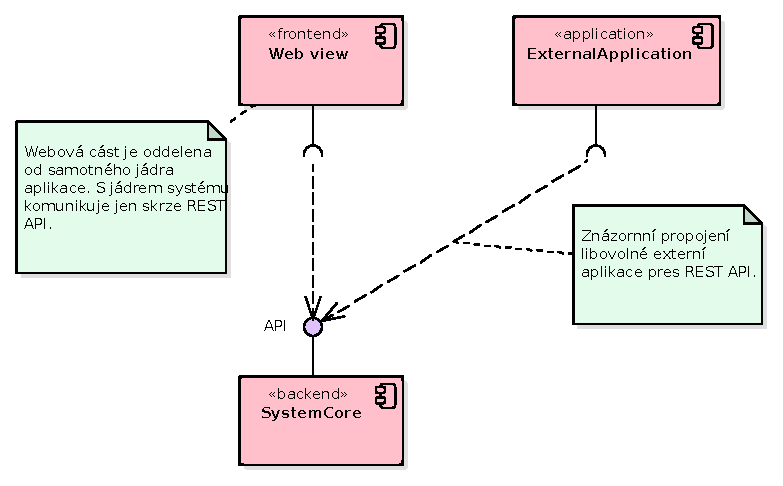
\includegraphics[width=1\textwidth]{Component_Model.pdf}
 	\caption[Základní části systému]{Diagram zobrazuje dvě základní části systému (jádro systému a webová, nebo jakákoliv jiná aplikace napojená na API)}\label{parts}
 \end{figure}
  
  \subsection{Jádro systému}  
  Jádro systému se skládá ze čtyř hlavních komponent, které lze také vidět na obrázku \ref{packages_core}. Pro administraci definic objektů slouží komponenta API. Další komponentou je Model, který obsahuje
  třídy využívané všemi komponentami. O načítání, ukládání a přístup k definicím objektů se stará komponenta Container.
  Poslední základní komponentou je Publisher, který zpřístupňuje celý systém klientovi v podobě vygenerovaných objektů.
  
  
  \begin{figure}\centering
 	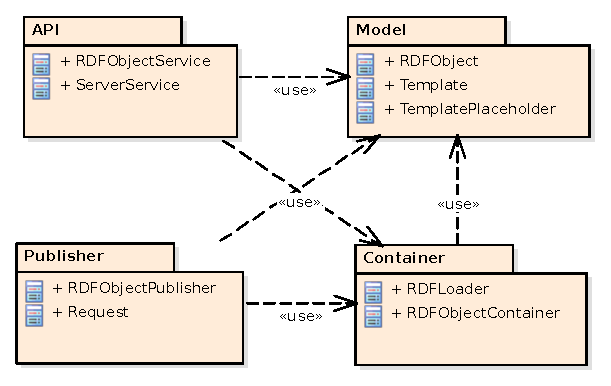
\includegraphics[width=0.8\textwidth]{Components.pdf}
 	\caption[Model komponent]{Základní čtyři komponenty jádra systému}\label{packages_core}
 \end{figure}
  
  \subsubsection{Komponenta API}\label{component_api}
    Tato komponenta slouží pro administraci definic objektů. Jedná se o komponentu, ke které má přístup pouze administrátor systému. Obsahuje dvě třídy, které
    mají své metody vystavené pro napojení přes API.
    
    Tyto třídy jsou zobrazeny na obrázku \ref{api_class}. Třída  \texttt{RDFObjectService} slouží k samotnému vytváření, úpravě a mazání definic.  
    Třída \texttt{ServerService} pak obsahuje
    metodu, která se dá taktéž volat přes API a slouží ke znovunačtení všech definic z nastaveného uložiště.
    \begin{figure}\centering
 	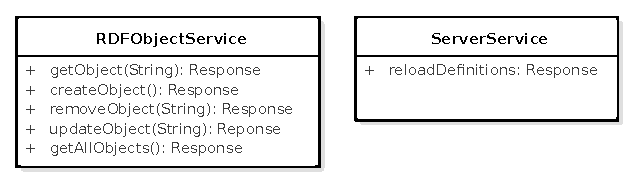
\includegraphics[width=0.8\textwidth]{API.pdf}
 	\caption[Model tříd API]{Třídy reprezentují služby, které mají metody vystavené pro API}\label{api_class}
    \end{figure}
    
    \subsubsection{Komponenta Model}\label{component_model}
    Tato komponenta obsahuje tři základní třídy, které jsou využívány zbytkem aplikace. Jedná se o třídy  \texttt{RDFObject},  \texttt{Template} a  \texttt{TemplatePlaceholder}, které jsou zobrazeny
    na obrázku \ref{model_class}.
    
     \begin{figure}\centering
	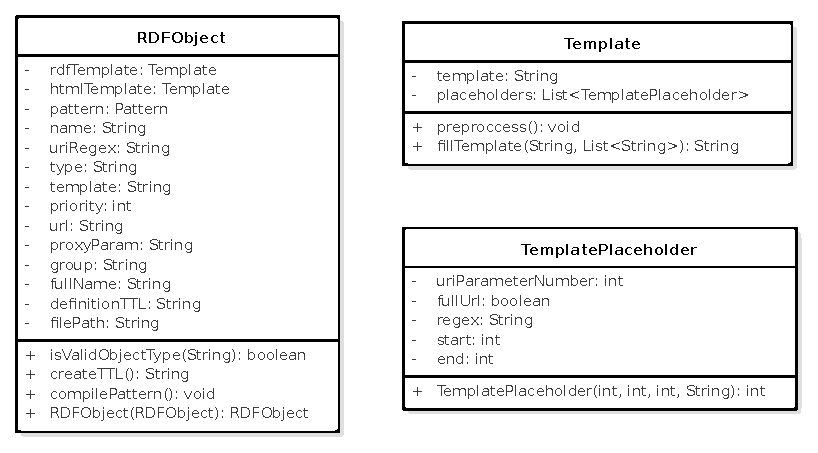
\includegraphics[width=\textwidth]{Model.pdf}
	\caption[Model tříd komponenty model]{Třídy v komponentě Model. Pro přehled jsou uvedeny pouze nejdůležitější metody. Třídy jinak obsahují i další metody, převážně settery a gettery.}\label{model_class}
    \end{figure}
    
    Třída  \texttt{RDFObject} reprezentuje samotnou definici objektu. Obsahuje dva atributy typu  \texttt{Template}.
    Prvním z nich je šablona definice (RDF serializace, nebo SPARQL dotaz) a
    druhou je HTML šablona sloužící pro zobrazení objektu v HTML formátu. Dále obsahuje metody jako jsou například validace a kompilace patternu
    regulárního výrazu pro pozdější identifikace definice dle požadavku klienta. Obsahuje také gettery a settery pro atributy, které ale nejsou
    na zmíněném diagramu vidět pro jejich primitivnost.
    
    Třídy  \texttt{Template} a  \texttt{TemplatePlaceholder} zastřešují celý šablonovací systém. Třída  \texttt{Template} obsahuje dvě důležité metody pro předzpracování šablony
    a následné vyplnění šablony při požadavku. Předzpracování šablony probíhá tak, že se v šabloně naleznou všechny placeholdery a uloží se do seznamu
    pro pozdější vyplnění. Předzpracování probíhá pouze jendou při nahrání definic (při startu serveru nebo znovunačtení definic). Cílem takto
    předzpracované šablony je urychlení generování objektů tak, aby se pouze dosazovaly hodnoty a případně aplikovaly podporované regulární výrazy.
 
 \subsubsection{Komponenta Container} \label{component_container}
 O správu nahraných definic se stará komponenta Container. Z obrázku \ref{container_class} je patrné, že obsahuje 2 třídy.
 
 Třída  \texttt{RDFLoader} se stará
 o čtení jednotlivých definic z file systému a následnou transformaci definice v Turtle formátu do objektu  \texttt{RDFObject},
 který reprezentuje konkrétní definice.
 
 Třída  \texttt{RDFObjectContainer} slouží jako kontejner (malá databáze) všech nahraných objektů. Objekty si drží jak podle celého jména definice pro rychlý přístup
 k definicím pro API, tak i podle priorit, podle kterých dochází k vyhledávání definic při požadavku klienta.
 Kontejner se v aplikaci vyskytuje díky použití singleton patternu
 pouze jeden a je nejvytíženějším objektem v celé aplikaci, protože je využíván všemi komponentami.
 
 \begin{figure}\centering
 	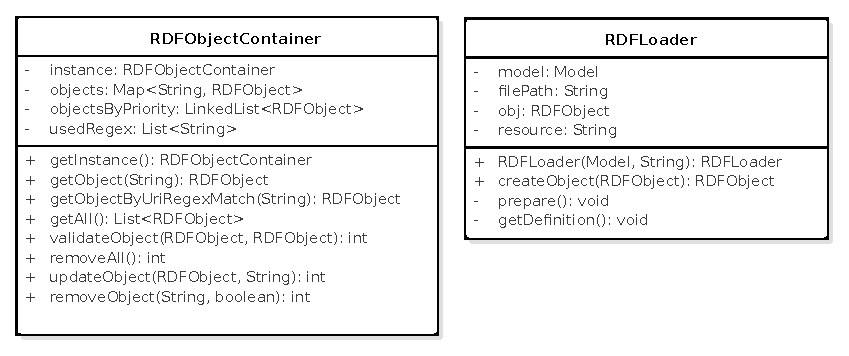
\includegraphics[width=\textwidth]{Container.pdf}
 	\caption[Model tříd komponenty container]{Komponenta container obsahuje třídy pro administraci objektů}\label{container_class}
    \end{figure}
    
    \subsubsection{Komponenta Publisher}\label{component_publisher}
    Tato komponenta slouží k odbavování požadavků klienta na vygenerování objektu. Na obrázku \ref{publisher_class} lze vidět 2 třídy,
    které mají za úkol interakci s klientem.
    
    Třída  \texttt{RDFObjectPublisherService} zpracovává prvotní požadavek klienta metodou \texttt{handleObjectRequest()}. V rámci systému je tato metoda definována
    pro všechny podporované serializace výstupu (HTML, RDF/XML, Turtle, JSON-LD a N-Triples). Při zavolání těchto metod je dále vytvořen 
    objekt třídy  \texttt{Request}, kterému je předána zodpovědnost za vygenerování výsledného objektu. 
    
    \begin{figure}\centering
 	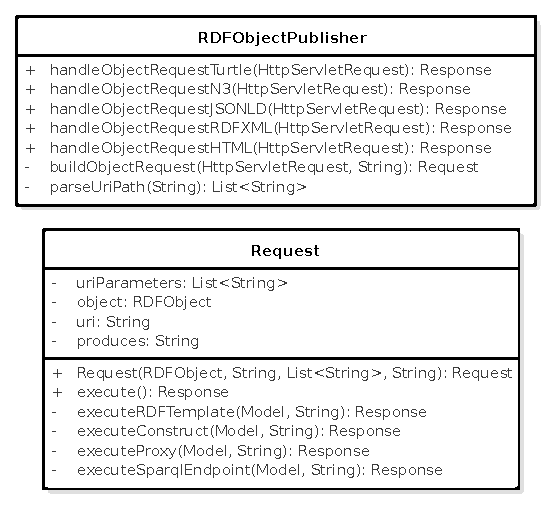
\includegraphics[width=0.8\textwidth]{Publisher.pdf}
 	\caption[Model tříd komponenty publisher]{Komponenta publisher obsahuje třídy pro zpracování požadavků klienta}\label{publisher_class}
    \end{figure}
    
    
   \newpage
   
   
 
 \section{Identifikace objektů, URL}
 \label{sec:identifikace}
 V kontextu RDF se dají objekty identifikovat pouze jedním způsobem, a to URL adresou. V tomto případě ale URL zastává ještě jednu důležitou úlohu.
 Vzhledem k tomu, že je jediným spojením mezi objektem (a jeho definicí) a vnějším prostředím, tak musí nést i informace, ze kterých bude později vygenerován
 konkrétní objekt. Návrhu struktury URL byla proto věnována velká pozornost.
 
 \subsection{Struktura URL v.1}
 Prvotní návrh byl takový, že se URL rozdělí na následující 3 části:
 \begin{itemize}
  \item Hostname
   \subitem Touto částí se rozumí identifikace serveru a protokolu, například \texttt{https://dynrdf.com}. Z pohledu objektu slouží jen jako část identifikátoru.
\newpage
    \item Identifikace objektu - první část cesty za hostname
     \subitem Tato část slouží k identifikaci objektu. Jedná se o unikátní název pro každý objekt. Příkladem může být například objekt časového intervalu s URL začínající 
     \texttt{https://dynrdf.com/time-interval}, kde \texttt{time-interval} identifikuje tento objekt.
     
    \item Parametry objektu
     \subitem Zbývající část URL nese informace, které se dosadí do šablon jednotlivých definic objektů. Jednotlivé parametry jsou vždy odděleny lomítkem.
     Například pro objekt ročního intervalu by mohla URL vypadat následovně \texttt{https://dynrdf.com/time-interval/2015/2016}, kde by zvolené roky znamenaly 
     parametry \texttt{od} a \texttt{do}.
 \end{itemize}
 Tento návrh by byl naprosto dostačujícím pro generování objektů všech podporovaných typů. Nicméně s sebou nese dva velké problémy.
 
 Prvním problémem je ten, že by musel být každý objekt identifikován IP adresou nebo doménou, kde tento server bude spuštěn. To by tedy znamenalo, že
 by tu nebyla možnost určit pro každý objekt extra URL v identifikátoru. Pokud by například funkce tohoto serveru chtěly využívat dvě různé společnosti, které
 by svoje objekty dále publikovali, tak by mohlo docházet k nekonzistenci odkazů na objekty. Jinými slovy se dá také zeptat na to, proč by nějaká společnost chtěla 
 publikovat data, kde jejich identifikace není spojena například s názvem společnosti. Vždy by v identifikaci figuroval tento server, který ale s původem dat nemá
 nic společného. Cílem tohoto systému je pouze generovat objekty a identifikaci a vlastnictví ponechat na autorovi daných definic objektů.
 
 Druhý problém, nebo spíše nepříjemnost nastavá v případě, že by se servery společností využívající tohoto dynamického generování chovali jako prostředníci 
 a požadavky na objekty přeposílaly na tento server. Pokud by každá definice měla vždy konkrétní unikátní identifikátor v URL adrese, pak by se pro každý takový objekt 
 muselo přidávat pravidlo ve webových serverech na přeposílání požadavku a případně i dál složitě parsovat URL z požadavku na primárním serveru na URL, která by byla 
 dle zmíněných specifikací.
 
 Pro lepší představu, jak může vypadat požadavek na konkrétní objekt přes prostředníka, třetí stranu, slouží obrázek \ref{request_flow_2}. Při požadavku
 přímo na tento server z klienta se proces na jiném serveru přeskočí. Ani jeden z těchto způsobů právě není bez nějakého výše zmíněného problému. 
 \begin{figure}\centering
 	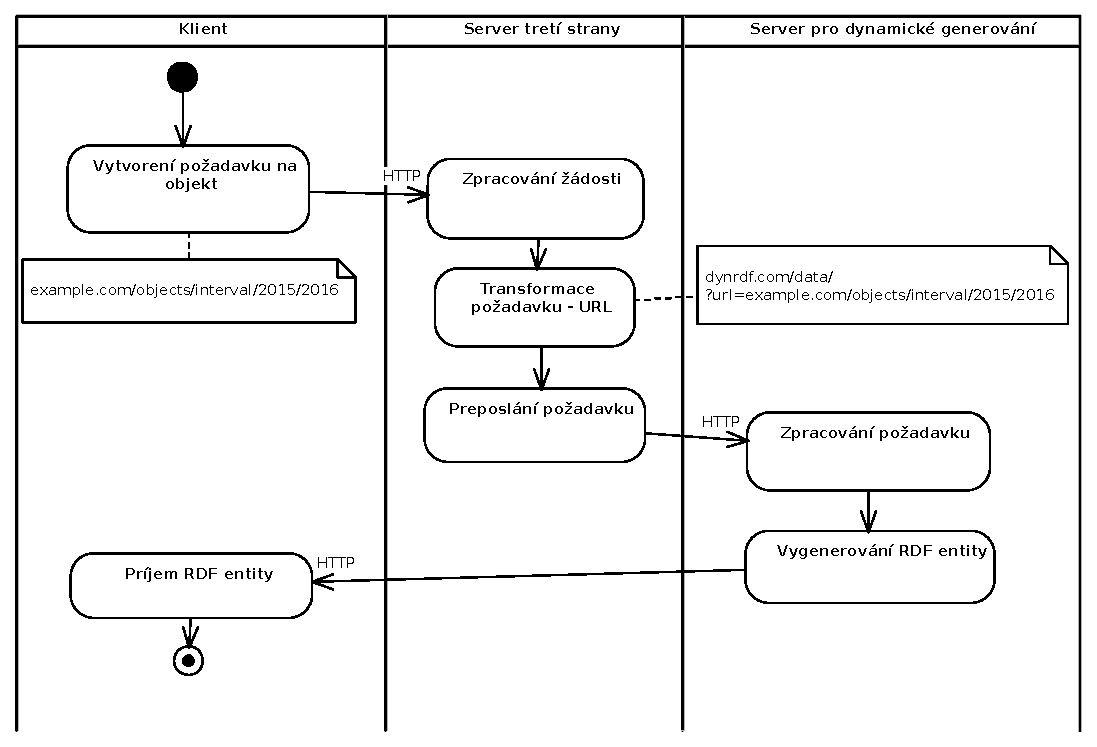
\includegraphics[width=1\textwidth]{request_flow}
 	\caption[Požadavek na objekt přes server třetí strany]{Požadavek na objekt přes server třetí strany. Prvotní návrh struktury URL adresy.}\label{request_flow_2}
 \end{figure}
 
 \subsection{Struktura URL v.2}
  Výše zmíněný návrh by znamenal téměř nepoužitelnost tohoto systému. Bylo proto nutné navrhnout jiné řešení. To se od původního návrhu liší na dvou místech, v předání
  informací o objektu a identifikací objektů.
  
  \subsubsection{Informace o objektu v GET parametru}
   Předání dat o objektu v GET parametru naprosto jednoduše řeší problém s parsováním URL adresy na serverech třetích stran. V případě, kdy na jiný server přijde požadavek
   na nějaký objekt, tak stačí v konfiguraci webových serverů nastavit pouze jedno pravidlo pro přeposlání požadavku pro všechny objekty.
  
  \subsubsection{Identifikace objektů, regulární výraz}
   Předání informací o objektu v GET parametru má ale za následek, že URL adresa už neobsahuje identifikátor objektu jako první část cesty. Objekt se dá identifikovat 
   pouze z informací v GET parametru, pro který účelově není stanovena žádná struktura.
   
   Strukturu URL adresy v GET parametru, která má identifikovat konkrétní objekt, zná pouze autor definice. Ideálním nástrojem, jak docílit mapování URL na konkrétní
   objekt je zde regulární výraz, kterému odpovídá konkrétní struktura požadavku.
   
\subsection{Shrnutí}
   Druhým návrhem struktury URL adresy se docílilo toho, že tento server bude schopný generovat objekty, jejichž identifikátor (URL) nebude závislý na adrese, kde tento
   server bude spuštěn.
   
   Příkladem může být například adresa \\ \texttt{http://dynrdf.com/?url=http://dataowner.com/objects/year/2015}. Původní požadavek mohl přijít na server, 
   který je uveden v parametru \texttt{url}. Tento požadavek byl následně přesměrován na tento server, kdy se za parametr dosadila 
   původní URL adresa požadavku. Následně se vygeneruje objekt roku 2015, jehož identifikátorem je obsah  \texttt{url} parametru.

   \newpage
   
 \section{Definice objektů}\label{obj_def}
  Každý objekt, který má být dynamicky generován tímto systémem, musí být nadefinován administrátorem a následně uložen.
  Základními atributy, které daná definice musí obsahovat jsou:
  \begin{itemize}
    \item název
      \subitem Název slouží k identifikaci objektu v rámci seznamu.
    \item skupina
      \subitem Skupina zde označuje například název společnosti, jméno autora, nebo jiný identifikátor autora dané definice objektu. 
      Společně s názvem tvoří plně kvalifikované jméno definice.
    \item URL regex
      \subitem Tento regulární výraz slouží k identifikaci konkrétní definice. Regulární výraz by měl popisovat URL adresy, pod kterými bude výsledná RDF entita
      dostupná.
    \item priorita objektu
      \subitem Priorita ovlivňuje pořadí definic, v jakém se pokouší systém najít shodu regulárního výrazu s příchozí URL. Některé regulární
      výrazy moho popisovat více objektů. Pokud je nějaký výraz více specifičtější než jiný, tak se zvýšením priority dané definice dosáhne k požadované shodě.
      Priorita se určuje celým číslem. Čím menší číslo, tím větší priorita a tím dříve se bude snažit systém najít shodu s příchozí adresou právě u dané definice.
      
    \item typ definice
      \subitem Typ definice označuje způsob zadání a vygenerování výsledného objektu. Konkrétním typům dle požadavku \ref{sec:object_types} se tento text věnuje dále.
    \item šablona objektu
      \subitem Šablonou se zde rozumí text vyplněný placeholdery, do kterých se při generování doplní hodnoty. Šablonou může být SPARQL dotaz nebo kterákoliv 
      podporovaná RDF serializace.
      
    \item HTML šablona
      \subitem Jedná se o podobnou šablonu jako pro konkrétní objekt, která je určena pro zobrazení ve webových prohlížečích.    
 \end{itemize}
 U některých typů jsou definovány výjimky, nebo další povinné atributy. Tyto specifikace jsou zmíněny dále u popisu těchto typů.
 
 Definice objektů přes Turtle formát musí splňovat RDF schéma, které je dostupné v příloženém souboru \texttt{dynrdf.rdfs.ttl}.
 
 \subsection{RDF serializace}
   Definice objektu, který je definovám šablonou v RDF formátu, musí obsahovat všechny zmíněné povinné atributy. Do RDF šablony jsou doplněny při generování parametry z
   URL a vyplněná šablona je poté už výsledným požadovaným objektem.
 
 \subsection{SPARQL Construct}\label{sparql_construct}
  Šablonou pro tento typ je SPARQL construct dotaz, kde se jednotlivé parametry bindují pomocí funkce \texttt{BIND()}. Tento typ definice díky jazyku 
  doplňuje RDF serializace o další funkcionality tohoto dotazovacího jazyka.
  
  Pro vygenerování objektu jsou zde zapotřebí 2 kroky. Dosazení parametrů do šablony jako v případě RDF serializace a následně spuštění SPARQL dotazu lokálně, který
  vytvoří požadovaný objekt.
  
 \subsection{SPARQL Endpoint}
  SPARQL je navržen pro dotazování se nad datasety. Tato data jsou dostupná přes služby běžící na SPARQL protokolu. Tento typ tedy slouží ke konstrukci
  komplikovanějších objektů, jejichž atributy mohou být výsledkem dalších \\SPARQL dotazů nad konkrétním datasetem. Výsledkem tohoto typu je RDF dokument construct
  nebo describe dotazu.
  
  Oproti lokálnímu construct dotazu se tento dotaz vykonává na jiném serveru. Proto je pro tento typ definice dalším povinným atributem URL adresa endpointu.
  
 \subsection{Proxy}
  Server má fungovat také jako prostředník mezi klientem a jinou aplikací poskytující RDF entity. Jinou aplikací se rozumí webová služba, na kterou se bude požadavek
  přeposílávat. Tyto aplikace nemusí implementovat překlad objektů do jiných RDF serializací. Překlad do požadovaných serializací funguje zde na serveru stejně jako
  pro ostatní objekty.
  
  Pro tento typ definice není potřeba definovat šablonu objektu, ale dalšími povinnými atributy jsou:
  \begin{itemize}
  \item proxy URL
    \subitem Jedná se o URL webové služby pro předaní zodpovědnosti za vygenerován objektu.
    
  \item název GET parametru
    \subitem Příchozí URL s informacemi o objektu je také přeposlána na danou službu. Názvem GET paramteru se rozumí parametr, do kterého se dosadí tato URL.
 \end{itemize}
 
 \section{Šablonovací systém}\label{template_system}
 Šablonovací systém je jedním ze stavebních kamenů této práce. Vyplněním šablony vzniká buď už konkrétní objekt, nebo SPARQL dotaz pro vygenerování objektu.
 Cílem návrhu tohoto systému je jednoduchost, ale zároveň dostatečná funkcionalita pro generování objektů různými způsoby.
 
 \subsection{Placeholder}
 Data o objektech jsou do šablon dosazeny přes placeholdery. Placeholderem se rozumí textový objekt, který definuje místo v dokumentu pro dosazení parametrů
 a má takovou strukturu, aby ho nebylo možné zaměnit s částí textu která nemá být nahrazena. V kontextu této práce se bude placeholderem rozumět textový objekt
 v tomto formátu:
 \begin{equation} \label{eq:placeholder}
 \texttt{[@<d>[, <regex>]]}
 \end{equation}
 
 Placeholder se skládá ze dvou částí. První povinnou částí je parametr \textit{\texttt{@<d>}}, který určuje konkrétní parametr URL adresy objektu,
 který se místo placeholderu dosadí. Jedná se tedy o \textit{vstup} do placeholderu.
 Druhým nepovinným parametrem je regulrní výraz, který se může aplikovat před dosazením textu na vstup placeholderu.
 
 \subsubsection{Vstup placeholderu}\label{placeholder_input}
 Jak bylo zmíněno v kapitole o identifikaci objektu \ref{sec:identifikace}, každý objekt je definován URL adresou, která je serveru předána GET parametrem.
 Pomocí informací, které obsahuje tato adresa, je potřeba vygenerovat konkrétní objekt.
 
 URL adresa je pro vstup do placeholderů rozdělena na části mezi lomítky. Na tyto části se dá odkazovat v placeholderu následujícím způsobem. Jako příklad 
 budou uvedeny reference k adrese\\ \texttt{http://intervals.com/year-interval/2013/2016}.
  
 \begin{itemize}
  \item @0 - reference na celou adresu\\(\texttt{http://intervals.com/year-interval/2013/2016})
  \item @1, @2, \ldots (kladné čísla za znakem \texttt{@}) jsou reference na pozice mezi lomítky URL adresy.
    \subitem @1 = \textit{http:}
    \subitem @2 = prázdný řetězec (mezi \texttt{//})
    \subitem @3 = \textit{intervals.com}
    \subitem @4, @5, @6 postupně \texttt{year-interval}, \texttt{2013} a \texttt{2016}
 \end{itemize}
 Tento způsob dává autorům šablon celkem snadný způsob, jak přímo z URL adresy dosadit do šablony požadované informace. Nicméně né všechny URL identifikátory objektů
 nemusí mít takovouto strukturu, aby se dalo snadno referencovat na konkrétní atributy objektu. Pokud by například v uvedeném příkladu nebyly roky rozděleny lomítkem,
 ale byly by v jednom parametru jako text \uv{\textit{2013-2016}}, nedal by se tento atribut rozdělit v RDF šabloně. Musel by se využít SPARQL construct dotaz, protože
 SPARQL obsahuje i funkce pro práci z řetězci (regulární výrazy). Proto je v placeholderu jako druhým nepovinným parametrem regulární výraz.
 
 \subsubsection{Regulární výraz v placeholderu}
  Pro možnost extrahování pouze části hodnoty parametru v šabloně slouží nepovinný atribut regulárního výrazu. Tento regulární výraz
  podporuje Capturing groups \cite{capture_group}. A to způsobem, kdy je ze vstupu placeholderu extrahována hodnota, která se nachází ve skupině číslo 1.
  
  Pokud by se autor šablony chtěl referencovat například na atribut \textit{@5} který by obsahoval\uv{\textit{2013-2016}}, 
  použil by jako placeholdery \texttt{[@5, ``(\textbackslash d+)-'']} pro \textit{2013}, resp. \texttt{[@5, ``-(\textbackslash d+)'']} pro \textit{2016}.
  Autoři šablon nebudou tedy nuceni používat SPARQL pro případy, kdy by potřebovali získat pouze část atributu, případně část z celé URL.
  
  \section{API}\label{api}
  API je další důležitou komponentou v aplikaci. Slouží pro ulehčení administrace definic a zároveň otevírá možnosti pro napojení externích
  aplikací do systému. 
  
  Prvotním návrhem API bylo pouze několik funkcí, které by zpracovávaly požadavky v JSON formátu pro základní CRUD
  operace. Vzhledem ale k tomu, že celá aplikace pracuje primárně v RDF formátech, byly tyto funkce rozšířeny i o další, které umožňují administraci
  objektů za pomoci definic v Turtle formátu. Jedná se o totožné soubory, které administrátor může nahrát do složky s definicemi objektů, odkud se 
  při startu nebo reloadu aplikace nahrají do systému. Výhodou tohoto kroku je i validace při požadavku na vytvoření nebo aktualizaci definice,
  která se u definic přímo vložených do složky provádí až při dalším spuštění nebo reloadu. Administrátor tedy může vidět chyby nebo možné konflikty
  ihned při pokusu o nahrání definice přes API a nemusí hledat v logu důvody, přoč byla jeho definice, kterou nahrál přímo do složky, odmítnuta.
  
  Celé API je rozdělené do dvou částí. Tou první je část pro zmíněnou administraci objektů, druhou pak API pro operace nad celým systémem.
  Nyní se počítá u systémového API pouze s funkcí pro znovunačtení definic ze složky pro ně určené. Pro tuto jedinou funkci by se API rozdělovat nemuselo,
  nicméně se počítá s dalším vývojem, kdy může být zapotřebí spravovat již běžící instanci serveru. Pro tyto operace už je vhodné rozdělit API na dvě části.
  
  \subsection{Struktura API}
  Pro administraci definic se v API využívá několik základních typů HTTP požadavků. Všechny operace také podporují vstup, respektive výstup v několika
  formátech. Stejně jako při požadavku klienta na konrétní objekt je zde využito principu Content negotiation.
  
  \subsubsection{Vytvoření objektu}
  Vytvoření objektu je možné jak ve formátu JSON, tak i v Turtle. Při vytváření objektu dochází také k validaci definice.
  Výsledek operace se klient dozví přes kód odpovědi (200 - úspěch, 400 - chyba). V případě neúspěchu je v odpovědi k dispozici i popis chyby.
  Parametry HTTP požadavku jsou následující:
  \begin{itemize}
   \item Cesta: \texttt{/api/objects}
   \item Typ požadavku: POST
   \item Content type: application/json, text/turtle
  \end{itemize}
  
  \subsubsection{Aktualizace objektu}
  Stejně jako při vytváření objektu je i změna objektu možná přes JSON i Turtle a provádí se také validace.
  Zde jsou parametry HTTP požadavku následující:
  \begin{itemize}
   \item Cesta: \texttt{/api/objects/<fullname>}
    \subitem \texttt{<fullname>} zde označuje řetězec ve formátu \texttt{<skupina>/<název>} (parametry definice)
   \item Typ požadavku: PUT
   \item Content type: application/json, text/turtle
  \end{itemize}

  \subsubsection{Smazání objektu}
  Parametry požadavku pro smazání jsou:
  \begin{itemize}
   \item Cesta: \texttt{/api/objects/<fullname>}
   \item Typ požadavku: DELETE
  \end{itemize}
  
  \subsubsection{Přístup k definicím}
  Klient si přes API může nechat zobrazit definici konkrétního objektu nebo celou sadu definic. Pro zobrazení si může také
  vybrat jakýkoliv z podporovaných formátů.
  Struktura požadavku je následující:
  \begin{itemize}
   \item Cesta: \texttt{/api/objects/[<fullname>]}
    \subitem Pokud chce uživatel získat konkrétní definici, tak za nepovinný parametr \texttt{<fullname>} dosadí stejně jako například u vytváření objektu
    celé jméno ve tvaru \texttt{<skupina>/<název>}. Pro zobrazení všech definic se tento parametr vynechá.
   \item Typ požadavku: GET
   \item Content type: libovolný z podporovaných (například text/turtle, application/n-triples \ldots)
  \end{itemize}
  
  \subsection{RDF schéma}
  Každá definice objektu má povinné atributy, které musí obsahovat. Pro popis těchto atributů, respektive celé definice, slouží RDF schéma (RDFS).
  RDF schéma je rozšířením RDF umožňující popsat konkrétní zdroje. V kontextu této aplikace se jedná o definice objektů.
  
  RDFS této aplikace popisuje definice jako objekty tříd konkrétních typů definic (RDF serializace, SPARQL Construct \ldots). Dále definuje atributy, jako jsou
  například \textit{dynrdf:priority} nebo \textit{dynrdf:regex}. Pokud autor neví, k čemu například tyto atributy slouží, může se podívat 
  do schématu a přečíst si například komentář ke konkrétnímu atributu. Schéma k definicím je možné zobrazit si v příloze pod názvem $dynrdf.rdfs.ttl$.
  
  
  
  \chapter{Implementace}
  Tato kapitola obsahuje popis implementační částí této práce. Implementace je rozdělena na části dle komponent jádra systému uvedených v návrhu \ref{packages_core}
  a implementaci webové aplikace pro administraci definic. Z velké většiny vychází implementace z návrhu, od kterého se více liší pouze při implementaci 
  optimalizovaného vyhledávání definic, jak je dále popsáno v kapitole Komponenta Container \ref{impl_container}.
  
  
  \section{Komponenta Model}
  V této kapitole je popsána implementace komponenty Model dle návrhu \ref{component_model}. 
  Tato komponenta obsahuje následující tři třídy:
  
  \begin{itemize}
   \item \texttt{RDFObject}
      \subitem Objekty této třídy reprezentují definice konkrétních objektů.   
   \item \texttt{Template}
      \subitem Tato třída zastřešuje šablonovací systém pro šablony v RDF serializacích, SPARQL dotazech a HTML šablony.
   \item \texttt{TemplatePlaceholder}
      \subitem Objekty této třídy reprezentují jednotlivé placeholdery v šablonách.
  \end{itemize}
  Implementace těchto tříd je popsána v dalších kapitolách. Třídy \texttt{Template} a \texttt{TemplatePlaceholder} jsou popsány společně v kapitole
  Šablonovací systém.
  
  \subsection{Třída RDFObject}
  Tato třída popisuje konkrétní definice objektů. Jedná se o třídu, která neobsahuje téměř žádnou logiku aplikace, protože se jedná opravdu pouze o model.
  Kromě běžných getterů a setterů obsahuje pouze jednu složitější metodu, která z atributů konkrétních objektů vytvoří ekvivalentní definici v Turtle formátu.
  Touto metodou je \texttt{createTTL()} a je využívána při vytváření nových definic při požadavcích v JSON formátu, jak je dále popsáno v kapitole o implementaci
  API \ref{impl_api}.
  
  \subsection{Šablonovací systém}
  Tato kapitola popisuje implementaci šablonovacího systému. Z komponenty Model se jedná o popis implementace tříd \texttt{Template} a \texttt{TemplatePlaceholder}.
  
  Třída \texttt{Template} dle návrhu \ref{component_model} obsahuje atributy \texttt{template}, ve kterém je při načtení definice do kontejneru uložen řetězec
  definované šablony a atribut \texttt{placeholders}, ve kterém jsou drženy objekty třídy \texttt{TemplatePlaceholder} po předzpracování šablony.
  
  Předzpracování šablony slouží ke zrychlení běhu systému pro generování RDF entit. Jedná se o metodu \texttt{preprocess()} \ref{list:preprocess}.
  
  \begin{lstlisting}[float=htb,caption={Metoda preprocess(): předzpracování šablony},label=list:preprocess]
public void preprocess(){
      if(template == null) return; // proxy
      Matcher matcher = templatePattern.matcher(template);
      while (matcher.find()) {
	  int start = matcher.start();
	  int end = matcher.end();
	  String regex = null;
	  int groups = matcher.groupCount();

	  // parameter number + regex
	  if( groups > 1 ){
	      regex = matcher.group(3);
	  }
	  int uriParameter = Integer.parseInt(matcher.group(1));

	  TemplatePlaceholder record = new TemplatePlaceholder(start,
	      end, uriParameter, regex);
	  placeholders.add(record);
      }
  }
\end{lstlisting}
  
  Tato metoda v definované šabloně hledá všechny placeholdery, ke kterým vytváří ekvivalentní objekty třídy \texttt{TemplatePlaceholder}.
  Placeholdery jsou nalezeny v šabloně s využitím knihovny pro regulární výrazy \texttt{java.util.regex}. 
  Regulární výraz, který popisuje strukturu placeholedru dle návrhu v kapitole Šablonovací systém \ref{template_system}, má následující strukturu:
  
     \begin{equation}\label{regex_impl}
  \texttt{\textbackslash[\textbackslash s*@(\textbackslash d+)\textbackslash s*(,\textbackslash s*[\textbackslash"|\textbackslash \textbackslash"](.*)[\textbackslash"|\textbackslash \textbackslash"])?\textbackslash s*\textbackslash]} 
 \end{equation}
 
 Tento regulární výraz popisuje následující placeholdery:
 \begin{itemize}
  \item \texttt{[@0]}, \texttt{[@1]}, \ldots
    \subitem Placeholder, do kterého je později dosazena část URL nazývaná $vstupem\ placeholderu$, která je popsána v samostané kapitole \ref{placeholder_input}.
	   Tuto strukturu popisuje první část regulárního výrazu: \texttt{@(\textbackslash d+)}.
  \item \texttt{[@0, "regex"]},  \texttt{[@0, \textbackslash "regex\textbackslash "]}, \ldots
    \subitem Dle návrhu lze ze vstupu placeholderu extrahovat část řetězce pro dosazení. Část za čárkou umožňuje definovat regulární výraz, který může obsahovat
    jednu skupinu, která se bude při generování dosazovat místo placeholderu. Regulární výraz palceholderu se nachází mezi uvozovkami, před kterými se může vyskytovat
    zpětné lomítko pro escapování uvozovek v RDF serializaci JSON-LD.
    \subitem Část placeholderu s regulárním výrazem popisuje část regulárního výrazu \ref{regex_impl}
    \texttt{(,\textbackslash s*[\textbackslash"|\textbackslash \textbackslash"](.*)[\textbackslash"|\textbackslash \textbackslash"])?}. Otazník na konci znamená,
    že se jedná o nepovinnou část.
    
 \end{itemize}
 
 V placeholderu se také může vyskytovat libovolný počet mezer, odřádkování či tabulátorů. Toho je v regulárním výrazu, který popisuje strukturu placeholderu, 
 docíleno speciálním znakem \texttt{\textbackslash s*}. Tento regulární výraz je i s příkladem pro ukázku dostupný na adrese \url{http://regexr.com/3ddcr}.
 
 V metodě \texttt{preprocess()} se využívá třída \texttt{Matcher} z knihovny\\ \texttt{java.util.regex}, která dle zadaného regulárního výrazu vyhledává
 v textu shody. Tyto shody, neboli nalezené placeholdery, jsou poté zpracovány. Jsou vytvořeny jejich ekvivalentní objekty třídy \texttt{TemplatePlaceholder}
 a jsou vloženy do seznamu placeholderů v k dané šabloně. Při požadavku klienta se poté pracuje hlavně nad seznamem těchto placeholderů a není už potřeba znovu vyhledávat
 každý placeholder v šabloně.
 
 Šablonovací systém se stará i o \textbf{vyplnění šablony} při požadavku klienta. Třída \texttt{Template} obsahuje metodu \texttt{fillTemplate()}, která má jako
 vstupy URl požadavku a seznam parametrů URL adresy (parametry jsou zde myšleny řetězce mezi lomítky v URL adrese).
 Vyplnění šablony se provádí dle algoritmu \ref{alg_fill_template}.
 
 \begin{algorithm}
\caption{Algoritmus vyplnění šablony při požadavku klienta}
\label{alg_fill_template}
\begin{algorithmic}[1]
\Procedure{Fill template}{}
\\
templateText := \textbf{copy} template.templateText \\
filledTemplate := ""

\For{\textbf{each} placeholder \textbf{in} template.placeholders } \\
\State filledTemplate .= templateText.substr(0, placeholder.start)
\State paramValue := URI.get(placeholder.paramNum)
\If{placeholder.regex is not null}
  \State filledTemplate .= paramValue.apply(placeholder.regex)
  \Else 
  \State filledTemplate .=  paramValue
\EndIf \\
\State templateText.remove(0, placeholder.end) 
\EndFor
\State filledTemplate .=  templateText \\
\State \Return filledTemplate
\EndProcedure
\end{algorithmic}
\end{algorithm}
  
  V tomto algorimtu se pro každý předzpracovaný placeholder dosazuje do výsledného řetězce text před daným placeholderem a poté samotná hodnota placeholderu po dosazení
  části URL adresy (případně se aplikuje regulární výraz na tuto hodnotu). Na konci je výsledný text doplněn o zbývající část textu šablony a vznikne
  zde už výsledná vyplněná šablona. Může se jednat jak o RDF serializaci, SPARQL dotaz, tak i o HTML kód. Tato vyplněná šablona je poté navrácena k dalšímu zpracování.
  
  V algoritmu \ref{alg_fill_template} jsou uvedeny parametry třídy \texttt{TemplatePalceholder} jako \texttt{start}, \texttt{end}, \texttt{regex} a \texttt{paramNum}.
  Ty dle návrhu \ref{component_model} popisují pozici placeholderu v šabloně, číslo parametru a případně regulární výraz placeholderu.
  
  \section{Komponenta Container}\label{impl_container}
  Komponenta Container slouží k manipulaci s definicemi objektů. Zahrnuje dle návrhu \ref{component_container} třídy \texttt{RDFLoader} a \texttt{RDFObjectContainer},
  které se starají o nahrání definic do aplikace, vyhledávání konkrétních definic apod.
  Tyto třídy jsou popsány v dalších kapitolách.
  
  \subsection{Třída RDFLoader}
  Tato třída se stará o načítání definic objektů ze souborového systému. Načtené definice poté zpracovává za pomoci knihovny Apache Jena \cite{jena} 
  a vytváří již konkrétní instance třídy \texttt{RDFObject}, které reprezentují dané definice.
  
  O načítání definic v Turtle formátu se stará rekurzivní metoda \ref{list:rec_load}, která prohledává každou
  podsložku ve složce pro uložení definic objektů.   
  
        \begin{lstlisting}[float,floatplacement=H,caption={Metoda pro vytváření ekvivalentních objektů definic z Turtle souborů. Nastavení hodnot definice se 
      provádí voláním metody setParam()},label=list:get_definition]
private void getDefinition() throws Exception{
    String queryString = "PREFIX dynrdf: <" + Config.ObjectRDFS + ">\n"
      + "PREFIX rdf: <http://www.w3.org/1999/02/22-rdf-syntax-ns#>\n"
      + "PREFIX rdfs: <http://www.w3.org/2000/01/rdf-schema#>\n"
      + "PREFIX owl:  <http://www.w3.org/2002/07/owl#>"
      + "PREFIX dcterms: <http://purl.org/dc/terms/>"
      + "SELECT ?type ?value  \n"
      + "WHERE \n"
      + "  { <" + resource + "> ?type ?value }" ;
    Query query = QueryFactory.create(queryString) ;
    try (QueryExecution qexec =
      QueryExecutionFactory.create(query, model)) {
	ResultSet results = qexec.execSelect() ;
	for ( ; results.hasNext() ; ) {
	    QuerySolution soln = results.nextSolution() ;

	    RDFNode n = soln.get("value") ; 
	    String val;
	    if(n.isResource()){
		val = n.asResource().toString();
	    }
	    else{
		val = ((Literal)n).getLexicalForm();
	    }

	    Resource typeRes = soln.getResource("type") ;
	    String type = typeRes.toString();

	    Log.debug("Found: type=" + type + ", val=" + val);
	    try{
		setParam(type, val);
	    }
	    catch(Exception ex){
		throw new Exception("Exception during reading" +
		  "and setting parameters of the RDFObject: "
		  + ex.getMessage());
	    }
	}
    }
  }
\end{lstlisting}

    \begin{lstlisting}[float=htb,caption={Metoda pro načítání definic ze souborového systému},label=list:rec_load]
public static List<File> findObjectsDefinitionsRec(File dir)
  throws IOException {
      List<File> definitions = new ArrayList<>();
      File[] files = dir.listFiles();
      if(files != null){
	  for (File file : files) {
	      if (file.isDirectory()) {
		  definitions.addAll(findObjectsDefinitionsRec(file));
	      } else {
		  String name = file.getName();
		  if(name.matches("^.*\\.ttl$")){
		      definitions.add(file);
		  }
	      }
	  }
      }
      else{
	  throw new IOException("Cannot read directory: " 
	      + dir.getAbsolutePath());
      }

      return definitions;
  }
\end{lstlisting}

Tato třída z nalezených definic vytváří ekvivalentní objekty třídy \texttt{RDFObject} reprezentující definice objektů v metodě \texttt{createObject()}.
  V této metodě nejdřív dochází k volání metody \texttt{prepare()}, která mimo jiné validuje pomocí SPARQL dotazů danou definici v Turtle formátu, a poté
  k zavolání metody \texttt{getDefinition()} \ref{list:get_definition}, která také za pomoci SPARQL dotazu a knihovny Jena vytváří objekt dané definice.
  Z knihovny Jena jsou zde použity třídy \texttt{Query}, \texttt{QueryExecution}, \texttt{QuerySolution} a další, které slouží k provedení SPARQL dotazu
  nad danou definicí v Turtle formátu.
  
  
  \subsection{Třída RDFObjectContainer}
  Tato třída je implementována jako jedináček (Singleton). V celé aplikaci je tedy k dispozici pouze jedna isntance této třídy, ke které lze přistupovat
  voláním metody \texttt{RDFObjectContainer.getInstance()}. Tento typ třídy byl zvolen proto, že tato třída slouží jako databáze všech nahraných definic
  objektů a cílem je minimalizovat paměťovou náročnost tím, že by se objekty definic (objekty třídy \texttt{RDFObject}) neukládají na více místech a neduplikují se.
  
  Třída je z většiny implementována dle návrhu \ref{component_container}. Liší se ale v systému vyhledávání definic dle priorit,
  jak je popsáno samostatně v kapitole \ref{ef_search}.
  
  \texttt{RDFObjectContainer} obsahuje několik atributů, které se vždy vážou na již vytvořené definice objektů. Každý z těchto atributů má jinou datovou strukturu
  vhodnou pro konkrétní účel. Mezi tyto atributy patří:
  \begin{itemize}
   \item \texttt{Map<String, RDFObject> objects}
    \subitem Tento kontejner slouží pro uložení objektů pod celým názvem. Je využíván při dotazován se na definice z API a při validaci nových definic,
    kdy jsou kontorovány na duplicitní názvy.
    
    \item \texttt{List<String> usedRegex}
      \subitem Tento list obsahuje seznam regulárních výrazů již nahraných definic do aplikace. Slouží pro validaci u vytváření nových definic, kdy je zakázáno,
	aby dvě rozdílné definice měly stejný regulární výraz.
	
    \item \texttt{Map<String, LinkedList<RDFObject>> groupPriority}
	\subitem V této mapě jsou uloženy definice objektů ve spojovém seznamu (pro účely priorit), který je mapován na názvy skupin jednotlivých definic.
	  Jedná se oproti návrhu o optimalizovanou verzi určenou k rychlejšímu vyhledávání definic při požadavku klienta. Touto optimalizací se zabývá kapitola \ref{ef_search}.
  \end{itemize}
  
  Třída \texttt{RDFObjectContainer} obsahuje především metody pro nahrání definic do kontejneru, aktualizaci, mazání a vyhledávání konkrétních definic.
  Tyto metody pracují se zmíněnými atributy. Pro příklad, jak tyto metody vypadají, je zde uvedena \ref{list:find_by_regex} metoda \texttt{getObjectByUriRegexMatch()}, která
  je volána při požadavku klienta a vyhledává definici, která by odpovídala požadované URL adrese. 
  
  Tato metoda nejdříve najde požadovanou skupinu, ve které by se 
  definice měla nacházet. Pokud tato skupina není součástí požadavku, je definice vyhledávána v základní skupině kterou reprezentuje prázdný řetězec.
  Konkrétní definice je vyhledávána průchodem seznamu, který je udržován dle priorit definic při vkládání a aktualizaci definic. U každé definice je příchozí URL
  porovnána vúči regulárnímu výrazu dané definice a pokud je nalezena shoda, je výsledná definice navrácena. V opačném případě je navrácena hodnota \texttt{null}.

      \begin{lstlisting}[float=htb,caption={Metoda pro vyhledání definice dle požadované URL adresy},label=list:find_by_regex]
/**
  * Get first RDF object from container by regex match
  * @param uri String
  * @param group String
  * @return RDFObject | null if not found
  */
public RDFObject getObjectByUriRegexMatch(String uri, String group){
    if(groupPriority.get(group) == null){
	// unknown group
	return null;
    }
    for( RDFObject o : groupPriority.get(group) ){

	Pattern pattern = o.getPattern();
	Matcher matcher = pattern.matcher(uri);
	if (matcher.find()) {
	    return new RDFObject(o); // return copy
	}
    }

    return null;
}
\end{lstlisting}
  
  \subsubsection{Zefektivnění vyhledávání dle atributu group}\label{ef_search}
  Součástí definice objektu \ref{obj_def} je atribut skupina (group). Tento atribut měl původně sloužit pouze k přesnější identifikaci definic, nicméně byl využit
  i k efektivnějšímu vyhledávání definic při požadavku klienta.
  
  V původním návrhu by se při každém požadavku klienta na vygenerování RDF entity musel v nejhorším případě procházet celý seznam vytvořených definic.
  Při průchodu tímto seznamem je porovnávána URL adresa s regulárním výrazem definic a pokud by k tomu mělo docházet u všech požadavků, jednalo by se o celkem pomalý proces.
  
  Oproti návrhu tedy byla přidána možnost zadat při požadavku v GET parametru i parametr \texttt{group} a tím vytyčit pouze malou část všech definic v systému.
  Při požadavku klienta je pak vyhledávána definice, která by odpovídala požadované URL adrese, pouze v seznamu definic dané skupiny. Vyhledávání konkrétní definice
  je tímto způsobem urychleno a aplikace tedy umožňuje zpracovat více požadavků. 
  
  Implementace třídy \texttt{RDFObjectContainer} se oproti návrhu \ref{component_container} liší v atributu \texttt{groupPriority}, který už není pouze spojovým seznamem
  dle priorit (původní atribut \texttt{objectsByPriority}), ale objekt třídy \texttt{Map}, díky kterému je na každou skupinu vyskytující se v apliakci
  namapován vlastní seznam definic dle priorit.
  
  Pro ověření výsledků byl také proveden test, který popisuje kapitola \ref{performance_test}.
      
  \section{Komponenta API}\label{impl_api}
  Komponenta API obsahuje dle návrhu \ref{component_api} třídy \texttt{RDFObjectService} a \texttt{ServerService}. Zodpovědností těchto tříd 
  je zpracovávat požadavky pro administraci objektů.
  
  Při implementaci API byly ve velkém množství využity dostupné anotace z balíčku \texttt{javax.ws.rs}. Díky těmto anotacím je výsledný kód velice čistý, protože
  nebylo zapotřebí vlastní logiky pro zpracování požadavků dle typu HTTP metod. Příklad \ref{list:api_create} ukazuje metodu \texttt{createObject()} včetně třídy,
  na kterou je díky použitým anotacím přesměrován požadavek na vytvoření nové definice z JSON formátu.
    
        \begin{lstlisting}[float=htb,caption={Příklad použití anotací při požadavku na vytvoření nové definice},label=list:api_create]
    
@Path("/objects")
public class RDFObjectService {

    @POST
    @Consumes("application/json")
    @Produces("application/json")
    public Response createObject(String o){
        try{
            RDFObjectContainer container = RDFObjectContainer.getInstance();

            container.createObject(new Gson().fromJson(o, RDFObject.class));
        }
        catch( Exception ex ){
            return returnError(ex.getMessage());
        }

        return returnOK("Created.");
    }
}
\end{lstlisting}
 
 \newpage
  Použité anotace mají následující význam:
  \begin{itemize}
   \item \texttt{@Path("/objects")} určuje cestu, na které jsou metody této třídy dostupné. Jedná se například o URL adresu
   \url{http://dyrdf.com/objects}. Pokud klient přistoupí na tuto adresu, tak je v této třídě vyhledána metoda dle následujících anotací, která má zpracovávat
   konkrétní požadavek klienta.
   
   \item \texttt{@POST} určuje HTTP metodu, kterou daná metoda zpracovává. Podobně existují i anotace \texttt{@GET}, \texttt{@PUT} a \texttt{@DELETE}.
   
   \item \texttt{@Consumes("application/json")} určuje, jaký \texttt{Content Type} \cite{content_type} metoda zpracovává. V tomto případě se jedná o 
   \texttt{application/json}.
   
   \item \texttt{@Produces("application/json")} určuje, v jakém formátu metoda poskytuje odpověď. Tuto hodnotu určuje parametr \texttt{Accept} v hlavičce HTTP požadavku.
  \end{itemize}
  
  Na metodu \texttt{createObject()} jsou ve výsledku mapovány požadavky, které obsahují a zároveň i požadují data v JSON formátu. Tyto požadavky musí být 
  zároveň typu POST. Uvnitř metody je nad kontejnerem pro uchování definic zavolána metoda se stejným jménem, které je předán už přímo objekt
  třídy \texttt{RDFObject}, který vytvořila knihovna Gson \cite{gson} z JSON řetězce.
 
  Podobných metod třída \texttt{RDFObjectService} obsahuje více. Oproti návrhu \ref{component_api} obsahuje pro každou metodu jako je \texttt{createObject()} 
  ekvivalentní metody, které ale odpovídají v jiných formátech, případně jiný formát akceptují.
  
  Třída \texttt{ServerService} obsahuje aktuálně pouze jednu metodu, na kterou je mapován požadavek na znovunačtení definic objektů. Tato funkcionalita
  byla implementována pro načtení definic, které uživatel při běhu aplikace vloží do složky s	 definicemi.
  
  \section{Komponenta Publisher}\label{impl_publisher}
  Komponenta Publisher obsahuje dle návrhu \ref{component_publisher} dvě třídy, které jsou zodpovědné za vyřízení požadavků klienta na vygenerování RDF entit.
  
  Třída \texttt{RDFObjectPublisherService} se chová velmi podobně jako API třída \texttt{RDFObjectService}.
  Zpracování požadavků je směrováno na metody pomocí anotací, které byly pospsány v kapitole Implementace API \ref{impl_api}.
  V těchto metodách, jak lze vidět na ukázce kódu \ref{list:publish_turtle}, se dále uvnitř volá metoda \texttt{buildObjectRequest()}, která se kontejneru dotazuje na konkrétní definici
  a následně vytvoří objekt třídy \texttt{Request}, na který je předána zodpovědnost za vygenerování. Uvedený příklad oproti metodám v API obsahuje navíc anotaci
  \texttt{@Context}, díky které je do parametrů metody injektován objekt třídy \texttt{HttpServletRequest}, ze kterého je možné přistupovat k obsahu HTTP požadavku.
  
  \begin{lstlisting}[float=htb,caption={Metoda pro zpracování požadavku klienta na vygenerování RDF entity v Turtle formátu},label=list:publish_turtle]
  @GET
  @Produces("text/turtle")
  public Response 
      handleObjectRequestTurtle(@Context HttpServletRequest request) {

      Request objectRequest;
      try{
	  objectRequest = buildObjectRequest(request, "TURTLE");
      }
      catch(RequestException ex){
	  return return4xx(ex.getMessage());
      }

      return objectRequest.execute();
  }
\end{lstlisting}
Funkcí uvedeného příkladu je zpracovávat požadavky na vygenerování RDF entit, které jako výstup očekávají Turtle formát. Zodpovědnost za vygenerování
je v těle metody předána třídě \texttt{Request}.
\newpage

Třída \texttt{Request} reprezentuje požadavky na už konkrétní RDF entity. Hlavní zodpovědností této třídy je na základě URL adresy a nalezené definice
vygenerovat výslednou RDF entitu. 

Tato třída obsahuje metody \texttt{executeConstruct()}, \texttt{executeProxy()} a další, jejichž úkolem je vygenerovat
výslednou entitu dle typu definice. Příklad \ref{list:construct_impl} ukazuje metodu pro generování RDF entity z definice typu SPARQL Construct \ref{sparql_construct}.
Vyplněná šablona obsahuje SPARQL Construct dotaz, který je pomocí třídy \texttt{QueryExecutionFactory	} vykonán. Výsledek dotazu je zapsán do modelu RDF Entity a na řádku 
\texttt{model.write(out, produces);} je serializován do zvolené RDF serializace, která je uložena v proměnné \texttt{produces}.

  \begin{lstlisting}[float=htb,caption={Metoda pro generování entit ze SPARQL Construct definicí},label=list:construct_impl]
private Response executeConstruct(Model model, String filledTemplate){
      try (QueryExecution qexec = QueryExecutionFactory
		      .create(filledTemplate, model)) {
	  model = qexec.execConstruct();
      }
      catch(Exception e){
	  return Response.status(404).build();
      }

      StringWriter out = new StringWriter();
      model.write(out, produces);

      return Response.status(200).entity(out.toString()).build();
  }
\end{lstlisting}
  
  \section{Webová aplikace pro administraci definic}\label{impl_web}
  Implementace webové aplikace je postavena na frameworku AngularJS \cite{angular}.
  Pro komunikaci s API byla implementována REST služba, která definuje chování frameworku při administraci definic. Tato služba je uvedena v příkladu \ref{list:ng_service}.
  V rámci této služby bylo potřeba pouze nastavit URL adresu API a HTTP metodu pro aktualizaci definic.
  
    \begin{lstlisting}[float=htb,caption={Služba pro komunikaci s API ve webové aplikaci. Proměná REST\_SERVICE je definovaná globálně a jejím obsahem je adresa serveru pro dynamické generování},label=list:ng_service]
angular.module('dynrdfApp.services',[])
  .factory('RDFObject',function($resource){
    return $resource(REST_SERVICE + 'objects/:id',{id:'@id'},{
        update: {
            method: 'PUT'
        }
    }
    );
})
\end{lstlisting}
  
  
  Aplikace obsahuje pouze dva kontrolery. \texttt{RDFObjectEntityController} se stará o tvorbu a aktualizaci definic a \texttt{OverviewController}
  o zobrazení již vytvořených definic klientovi. 
  Implementace těchto kontrolerů je uložena v příloze ve zdrojových kódech v souboru \texttt{src/main/webapp/js/controllers.js}.
  
  Pro vizuální část aplikace byl použit front-endový framework Bootstrap \cite{bootstrap}.
  
  
  \chapter{Testování}  
  Cílem testování této aplikace je ověřit celkovou funkčnost systému.  
  Při úpravách zdrojových kódů může dojít k ovlivnění chování již implementovaných metod
  a tudíž k neočekávanému chování celé aplikace. Nestandartní chování může také ovlivnit prostředí (např. jiná verze Javy), ve kterém je aplikace spuštěna.
  Cílem testů je toto nestandartní chování odhalit a upozornit na něj vývojáře s cílem aby toto chování analyzoval a opravil.
  
  Jedním typem testování jsou testy implementovaných funkcí přes \textbf{unit testy} a \textbf{integrační testy}.
  Druhým typem testů je \textbf{testování výkonu}. Testování aplikace dle těchto typů je popsáno v následujících kapitolách.
    
  \section{Unit testy}
  Unit testy slouží k otestování správné funkčnosti jednotlivých částí systému. 
  V této aplikaci jsou tímto způsobem testovány nejvíce metody tříd \texttt{Template} \ref{component_model} a \texttt{RDFObjectContainer} \ref{component_container}.
  Ostatní třídy jsou testovány na úrovni integračních testů.
  
  \subsection{Testy třídy Template}
  Třída Template pracuje s šablonami jednotlivých definic. Nerozlišuje přitom, zda se jedná o HTML šablonu nebo například o šablonu v Turtle serializaci.
  Tato třída obsahuje 2 metody - \texttt{preprocess()}, která vyhledává a ukládá si pro další použití informace o placeholderech v šabloně a metoda
  \texttt{fillTemplate()}, která vyplňuje šablonu při požadavku klienta.
  
  Testy těchto metod jsou obsaženy ve třídě \texttt{TemplateTest}. Příkladem jednoho z testů je test na vyplnění šablony včetně extrahování
  části URL adresy díky regulárnímu výrazu.
  V tomto testu \ref{list:test_template} je vytvořena šablona obsahující pouze jeden placeholder s regulárním výrazem, který z 
  URL adresy extrahuje část za řetězcem \texttt{http://}.
  Testovanou URL adresou je zde \texttt{http://test.com/a/b/c} a výsledný řetezec po vyplnění šablony je testován na obsah \texttt{test.com/a/b/c}.
  
  \begin{lstlisting}[float=htb,caption={Unit test na vyplnění placeholderu v šabloně s regulárním výrazem},label=list:test_template]
  @Test
  public void testRegexTemplate(){
      String plainTemplate = "[@0, \"http://(.*)\"]";
      Template template = new Template(plainTemplate);
      template.preprocess();
      Assert.assertEquals(1, template.getPlaceholders().size());
      String testUrl = "http://test.com/a/b/c";
      String filledTemplate = template.fillTemplate(testUrl,
	Arrays.asList(testUrl.split("/")));

      String expected = "test.com/a/b/c";
      Assert.assertEquals(expected, filledTemplate);
  }
\end{lstlisting}
  
  \subsection{Testy třídy RDFObjectContainer}
  Třída RDFObjectContainer \ref{component_container} obsahuje metody pro manipulaci s definicemi objektů, jako je přidání, smazání,
  aktualizace a také validaci těchto definic.
  Ke každé z těchto metod jsou napsány testy ve třídě\\
  \texttt{RDFObjectContainerTest}, které ověřují jejich funkcionalitu. Validační testy pokrývají všechny typy nevalidních definic, jako jsou duplicitní
  celé názvy definic (stejná skupina a název), chybějící parametry, nevalidní URL například pro Proxy objekt aj.  
  Pro testování těchto funkcionalit jsou předpřipravené definice v adresáři \texttt{textObjects}.
  
  Příkladem těchto testů je například validační test na špatnou strukturu URL adresy \ref{list:test_url}, která v tomto případě neobsahuje protokol, nebo test
  pro přidání definice do kontejneru \ref{list:test_create}, který definici vytvoří a přidá do kontejneru a poté se ho snaží získat zpět.
  
    \begin{lstlisting}[float=htb,caption={Unit test třídy RDFObjectContainer: Malformed URL},label=list:test_url]
  @Test(expected = ContainerException.class)
  public void validateProxyMalformedUrl() throws ContainerException{
     RDFObjectContainer container = RDFObjectContainer.getInstance();
     // missing protocol - URL validator is set to check protocol
     RDFObject o = new RDFObject("name", "tests", "validations",
       "PROXY", "empty template", 1, "test.com", "param", "html", null);

     container.validateObject(o, false, null);
  }
    
\end{lstlisting}

\begin{lstlisting}[float=htb,caption={Unit test třídy RDFObjectContainer: Vytvoření a vložení definice},label=list:test_create]
  @Test
  public void testCreate(){
      RDFObjectContainer container = RDFObjectContainer.getInstance();
      RDFObject o = new RDFObject("createTestContainer", "tests",
	"createTestContainer", "TURTLE", "empty template", 1,
	"", "", "html", null);
      boolean ok = true;
      try{
	  container.createObject(o);
      }
      catch(Exception ex){
	  ok = false;
      }
      Assert.assertTrue(ok);
      Assert.assertNotNull(container.getObject(o.getFullName()));
  }
    
\end{lstlisting}
  
    
  
  \section{Integrační testy}
  Integrační testy slouží k testování funkčnosti více komponent dohromady. V rámci této aplikace se jedná o komponenty dle návrhu \ref{packages_core} 
  (komponenty API, Model, Container a Publisher). Pro úspěšné spuštění integračních testů je potřeba připojení k internetu, protože se testuje i generování
  RDF entit u definic typů Proxy a SPARQL Endpoint, které se připojují ke SAPRQL Endpointu portálu DBpedia na adrese \url{http://dbpedia.org/sparql}.
  Pro tyto testy se používají testovací definice dostupné v příloze v adresáři \texttt{testObjects}.
  
  \subsection{Testy třídy Request}
  Třída \texttt{Request} \ref{publisher_class} má na starost zpracování požadavku klienta na vygenerování už konkrétní RDF entity. Obsahuje metody
  pro vygenerování entit, jako jsou
  \texttt{executeProxy()}, \texttt{executeRDFTemplate()} a další dle typů definice. Cílem testů pro tuto třídu je ověřit integraci s ostatními komponentami
  pro generování RDF entit.   
  Každý typ definice je testován na všechny podporované výstupní serializace.
  
  Jako příklad \ref{list:test_execute_endpoint} je zde uveden test metody \texttt{executeSPARQLEndpoint()}, který ověřuje funkčnost generování objektu typu SPARQL Endpoint.
  Při tomto testu dochází uvnitř aplikace ke komunikaci se serverem DBpedia, což je určeno testovanou definicí \texttt{loggerEndpoint}, která je k dispozici v příloze
  v adresáři \texttt{testObjects/logger\_endpoint.ttl}. Před provedením tohoto testu je inicializován kontejner a jsou do něj nahrány testovací definice. 
  V rámci tohoto testu se ověřuje, zda kontejner obsahuje danou definici a IRI vygenerované entity se shoduje s očekávaným identifikátorem nastavený v dané definici.
  Testování ostatních metod je velice podobné tomuto testu.
  
  \begin{lstlisting}[float=htb,caption={Test metody executeSPARQLEndpoint()},label=list:test_execute_endpoint]
@Test
public void testRequestExecuteSPARQLEndpoint(){
    RDFObject o = RDFObjectContainer.getInstance()
		  .getObject("dynrdf/loggerEndpoint");
    Assert.assertNotNull(o);

    String uri = "http://logservice.com/data/loggerEndpoint/" + 
		  "42/2016-05-01/10:00:23/org.dynrdf.Request/" +
		  "some exception msg";
    List<String> params = new ArrayList<String>(
	    Arrays.asList(uri.split("/")));
    Request request = new Request(o, uri, params, "TURTLE");
    Response r = request.execute();

    Assert.assertEquals(200, r.getStatus());
    String result = (String)r.getEntity();

    StringReader sr = new StringReader(result);
    Model model = ModelFactory.createDefaultModel();
    model.read(sr, null, "TURTLE");

    String res = selectresource(model);
    Assert.assertEquals("http://logservice.com/data/loggerEndpoint#42",
			res);
}
    
\end{lstlisting}

\subsection{Testy komponent API a Publisher}
Cílem testů těchto komponent je ověřit funkčnost samotných HTTP požadavků pro administraci objektů a požadavky na RDF entity.
Testování těchto komponent je prováděno we webovém kontejneru, který je spuštěn díky
testovacímu frameworku Jersey Test \cite{jersey_test} před každým testem.

Komponenta API \ref{api_class} obsahuje třídy \texttt{RDFObjectService}, která se stará o zpracování HTTP požadavků administrace definic,
a třídu \texttt{ServerService} která obsahuje zatím pouze metodu \texttt{reloadDefinitions()} pro znovu nahrání definic do systému.
Všechny metody, respektive všechny požadavky, které jsou na tyto metody mapovány, jsou testovány vůči testovacím definicím dostupných v příloze
v adresáři \texttt{testObjects}. 

Příkladem testu API je test \ref{list:test_api_create_json} na vytvoření definice, který posílá
informace o definici v JSON formátu. Otestováním tohoto požadavku je ověřena funkčnost požadavku na vytvoření definice z webové aplikace,
ta odesílá data v JSON formátech. V tomto testu je neprve vytvořen z objektu definice požadavek na vytvoření, který je poté odeslán. Následuje požadavek
na získání definice tohoto objektu ze serveru, který je kontrolován na úspěch (status kód 200).
  \begin{lstlisting}[float=htb,caption={Test vytvoření definice přes API v JSON formátu},label=list:test_api_create_json]
@Test
public void testCreateJson() {
    RDFObject o = new RDFObject("testobj1", "tests", "testobj1","
				"TURTLE", "empty template", 1,
				"", "", "html", null);

    final Response res = target("objects").request()
	      .post(Entity.entity(o, MediaType.APPLICATION_JSON_TYPE));
    Assert.assertEquals(200, res.getStatusInfo().getStatusCode());
    // get object
    final Response resGet = target("objects/" + o.getFullName())
	      .request(MediaType.APPLICATION_JSON_TYPE).get();
    Assert.assertEquals(200, resGet.getStatusInfo().getStatusCode());
}
    
\end{lstlisting}

V rámci komponenty Publisher jsou testovány metody třídy \\ \texttt{RDFObjectPublisherService}. Ty zpracovávají požadavky na konkrétní RDF entity.
Testování této třídy má za cíl ověřit funkčnost generování entit všech typů pro všechny podporované výstupní RDF serializace.

  
  \section{Testování výkonu}\label{performance_test}
  Cílem testování výkonu je zjistit, kolik požadavků za sekundu je tato aplikace schopna odbavit a s jakou dobou odpovědi.
  Na tyto hodnoty není předem kladen požadavek, který by aplikace
  musela splňovat. Jedná se o orientační test.
  
  Testování výkonu bylo provedeno aplikací Apache JMeter \cite{jmeter}. Aplikace byla pro tyto účely nasazena do webového kontejneru Glassfish 4.1.1 \cite{glassfish}
  na VPS s těmito parametry:
  \begin{itemize}
   \item Kontejnerová virtualizace OpenVZ
   \item CPU Intel(R) Xeon(R) E5-2630 @2.30GHz (8 virt. jader)
   \item 4GB RAM
   \item Ubuntu server 14.04
   \item Konektivita 300 Mbps
  \end{itemize}
  
  Testování probíhalo ze zařízení s těmito parametry:
  \begin{itemize}
   \item CPU Intel(R) Core(TM) i5-2410M @2.30GHz
   \item 8GB RAM
   \item OS Ubuntu 12.04
  \end{itemize}
  
  Sledovaným parametrem byla převážně propustnost (throughput). U ostatních parametrů, jako jsou například průměrná doba odpovědi, mohlo docházet ke zkreslení
  testu. Throughput je oproti těmto atributům testu více imunní na výkyvy, protože je vypočítáván algoritmicky a je brán v potaz například počet spuštěných
  testů na testovacím stroji.
  
  
  Při testování výkonu byly testovány všechny typy definic. Poměr definic typů RDF serializací vůči ostatním typům byl trojnásobný, protože se předpokládá
  s větším využitím definic tohoto typu.
  
  Těmito testy se ověřovalo také efektivnější vyhledávání při použití parametru \texttt{group} v URL adrese. 
  Tato optimalizace je popsána v kapitole implementace - RDFObjectContainer \ref{ef_search}.
  Testovány byly dva případy. 
  V prvním případě, jehož výsledky jsou uvedeny v tabulce \ref{performance1}, byly testovány dotazy včetně parametru \texttt{group}
  v URL adrese. Při druhém testu, jehož výsledky ukazuje tabulka \ref{performance2}, byl tento parametr vynechán.
  
  Testy výkonu ukázaly poměrně velký rozdíl mezi testovanými případy. Tím bylo ověřeno, že zmíněná optimalizace byla poměrně důležitým optimalizačním krokem.
  Při předpokladu, že některé požadavky na vygenerování RDF entit nebudou obsahovat zmiňovaný parametr \texttt{group}, je výsledný počet požadavků za sekundu
  větší než 100. Tento výsledek je na dané konfiguraci vyhodnocen jako postačující.
  
    
  \begin{table}\centering
 	\caption[Test výkonu - s parametrem group]{Test výkonu s parametrem group. Celková propustnost při tomto testu byla 147 požadavků za sekundu. Sloupce average, median, min a max označují trvání požadavku v ms po připojení.}\label{performance1}
 	\begin{tabular}{|l|r|r|r|r|r|r|r|}\hline
\textbf{Label}		& 	\textbf{Samples}&		\textbf{Median} &\textbf{Min} &	\textbf{Max} &		\textbf{Throughput} \tabularnewline \hline \hline
 Turtle			&	300	&			22&	10 &	5138&		29.8\tabularnewline \hline
 RDF/XML 		&	300	&			19&	9&	991	&	56.3\tabularnewline \hline
 NTriples 		&	300	&			24&	9&	5132 	&	31.6\tabularnewline \hline
 JSON-LD 		&	300	&			87&	9&	5141 	&	33.8\tabularnewline \hline
 SPARQL Construct 	&	100	&			36&	13&	950 	&	32.3\tabularnewline \hline
 SPARQL Endpoint 	&	100	&			315&	89&	5190 	&	13.5\tabularnewline \hline
 Proxy 			&	100	&			765&	325&	5212 	&	13.1\tabularnewline \hline
TOTAL			&	1500	&			29&	9&	5212 	&	147\tabularnewline \hline
 	\end{tabular}
 \end{table}
 
   \begin{table}\centering
 	\caption[Test výkonu - bez parametru group]{Test výkonu bez parametru group. Celková propustnost při tomto testu byla přibližně 91 požadavků za sekundu. Sloupce average, median, min a max označují trvání požadavku v ms po připojení.}\label{performance2}
 	\begin{tabular}{|l|r|r|r|r|r|r|r|}\hline
\textbf{Label}			& 	\textbf{Samples}&		\textbf{Median} &\textbf{Min} &	\textbf{Max} &		\textbf{Throughput} \tabularnewline \hline \hline
 Turtle				&300		&1549	&98	&5483	&19\tabularnewline \hline
 RDF/XML 			&300		&922	&134	&5419	&21.2\tabularnewline \hline
 NTriples 			&300		&3539	&232	&5527	&19.4\tabularnewline \hline
 JSON-LD 			&300		&4063	&970	&5503	&20.4\tabularnewline \hline
 SPARQL Construct 		&100		&3979	&1829	&5467	&8.4\tabularnewline \hline
 SPARQL Endpoint 		&100		&3936	&3490	&4518	&8\tabularnewline \hline
 Proxy 				&100		&4306	&3244	&5159	&7.5\tabularnewline \hline
TOTAL				&1500		&3596	&98	&5527	&91.4\tabularnewline \hline
 	\end{tabular}
 \end{table}
  
  
  \chapter{Uživatelská dokumentace}
  Tato kapitola obsahuje dokumentaci k vyvíjené aplikaci. Touto aplikací je webový server pro poskytování dynamicky generovanýcý objektů v RDF \cite{rdf} formátech.	
  
  Cílem této aplikace je uživatelům usnadnit tvorbu objektů v RDF formátech pomocí jednotných šablon pro výsledné RDF entity.
  Generování RDF entit přes tuto aplikaci má tyto výhody:
  \begin{itemize}
   \item \textbf{Jedna šablona pro mnoho objektů} 
   
   Uživatel může vytvořit jednu definici s šablonou pro mnoho (až nekonečně mnoho) podobných RDF entit, které se liší pouze v hodnotách atributů,
   ale strukturu mají stejnou (nebo velmi podobnou).
   
   \item \textbf{Malá kapacita uložišť}   
   
   Díky jednotné šabloně pro mnoho RDF entit není potřeba investovat do velkých úložných prostorů. Zapotřebí je mít pouze kapacity pro uložení
   definic těchto objektů, které jsou v porovnání s ukládáním všech RDF entit minimální.
   
   \item \textbf{Čas pro údržbu}
   
   Tato aplikace také šetří čas uživatelů při údržbě již publikovaných RDF entit. Pokud chce uživatel něco změnit v publikovaných RDF entitách, nemusí tak dělat
   pro každou entitu zvlášť, ale stačí pouze změnit šablonu na jednom místě a tato změna se automaticky promítne do všech výsledných RDF entit při
   dalším požadavku klienta.
      
  \end{itemize}

  V této aplikaci je uživateli umožněno nadefinovat si vlastní RDF entity a vytvořit si k nim
  šablony, ze kterých jsou následně dynamicky generovány dle příchozí URL. K administraci definic slouží webová aplikace a API.
  Klientovi jsou výsledné entity dostupné v několika RDF serializacích (Turtle, N-Triples, JSON-LD a RDF/XML) a jako webová stránka (HTML dokument).
  
   
  
  
  \section{Webová aplikace}\label{web_app}
  Pro administraci definic může uživatel využít webovou aplikaci. V této aplikaci je mu umožněno zobrazit si
  seznam definic, vytvářet, upravovat nebo smazat tyto definice.
  
  \subsection{Přehled definic}
  Při přístupu na hlavní stránku webové aplikace je uživateli k dispozici seznam již vytvořených definic. U každé definice se vyskytují dvě tlačítka - pro 
  zobrazení definice (a následnou editaci) a pro smazání definice.
  Pro založení nové definice může uživatel kliknout na tlačítko \uv{Add new object definition} a aplikace ho přesměruje na stránku s formulářem pro založení nové definice.
  Hlavní stránku s přehledem lze vidět na obrázku \ref{web_overview}
  \begin{figure}\centering
 	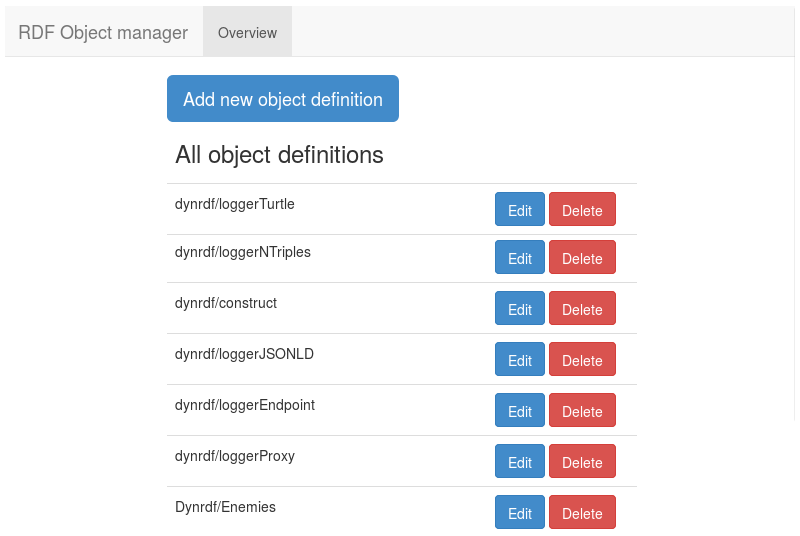
\includegraphics[width=\textwidth]{web_overview}
 	\caption[Přehled definic ve webové aplikaci - hlavní stránka]{Přehled definic ve webové aplikaci - hlavní stránka}\label{web_overview}		
  \end{figure}
    
    \subsection{Vytvoření nové definice}\label{def_create}
    Po kliknutí na tlačítko \uv{Add new object definition} je uživatel přesměrován na formulář pro založení nové definice. Tento formulář je zobrazen na obrázku
    \ref{web_create}.
    Uživatel zde nastavuje všechny atributy pro generování objektů.
    Ke každému atributu je na stránce také k dispozici nápověda, která se uživateli zobrazí po kliknutí na obrázek otazníku.
    Těmito atributy jsou:
    \begin{itemize}
     \item Název definice a skupina
      \subitem Název a skupina tvoří dohromady celé jméno definice ve formátu \textit{<skupina>/<název>}. Toto označení definice musí být v celém systému 
      unikátní. Uživatel může pojmenovat více definic stejným jménem, ale tyto definice musí mít rozdílné skupiny.
      
      Zavedení parametru $skupina$ má také výkonostní důvody, které jsou popsány v kapitole Přístup k objektům \ref{obj_access}.
      
      \item Regulární výraz
	\subitem Konkrétní definice jsou v systému identifikovány regulárním výrazem. Při požadavku klienta na konkrétní RDF entitu se server pokouší najít v 
	definicích regulární výraz, který požadované URL adrese odpovídá. Pokud tuto definici nalezne, tak podle ní výslednou entitu vygeneruje.
	
	Například URL adresa \url{http://company.com/objects/time/year/2016} odpovídá regulárnímu výrazu
	\uv{\texttt{\textbackslash /objects\textbackslash /time}}, což
	je možné vyzkoušet si i online na adrese \url{http://regexr.com/3dddd}.
	Pokud požadavek klienta obsahuje tuto URL adresu a v systému existuje definice s daným regulárním výrazem, je výsledný objekt vygenerován
	dle této definice.
	
	
      \item Priorita
	\subitem Tento atribut určuje pořadí definic, ve kterém bude systém hledat odpovídající definici při požadavku klienta. 
	Mezi jednotlivými definicemi může docházet ke konfliktům regulárních výrazů. Tyto výrazy nemusí být stejné, ale mohou popisovat velmi podobné struktury.
	Při nedefinovaném pořadí vyhledávání v definicích může docházet k nalezení shody u špatných definic a tudíž k vygenerování špatného objektu.
	Nastavením správných priorit lze tomuto problému alespoň zčástí předcházet. Definice jsou prohledávány v pořadí od nejvyšší (1) priority po nejmenší.
	
      \item Typ definice
	\subitem Typ definice určuje, jak bude generování objektu probíhat. Aplikace podporuje několik typů definic. Jedná se o RDF serializace (Turtle, JSON-LD, 
	N-Triples a RDF/XML), SPARQL dotazy (lokální Construct, nebo Construct/Describe dotaz na SPARQL endpointu) a typ Proxy, 
	který funguje na principu přeposílání požadavků.
	Všechny tyto typy jsou dále popsány v kapitole Typy definic \ref{def_types}
	\newpage
    \item Šablona definice
      \subitem Typ šablony závisí na typu definice. U RDF serializací se jedná o šablonu v konkrétní serializaci, zatímco u SPARQL typů
      se jedná o SPARQL dotaz. V šablonách se mohou využívat placeholdery pro dosazení parametrů z URL adresy. Šablonovací systém včetně formátu je popsán v kapitole
      Šablonovací systém \ref{template_system}. U typu Proxy se tento atribut nevyplňuje.
      
      \item HTML šablona
      \subitem HTML šablona slouží pro zobrazení dat o objektu v HTML formátu při požadavku z webových prohlížečů. Stejně jako u šablony definice se mohou využívat
      placeholdery pro dosazení parametrů z URL adresy.	
	
    \end{itemize}
    \begin{figure}\centering
 	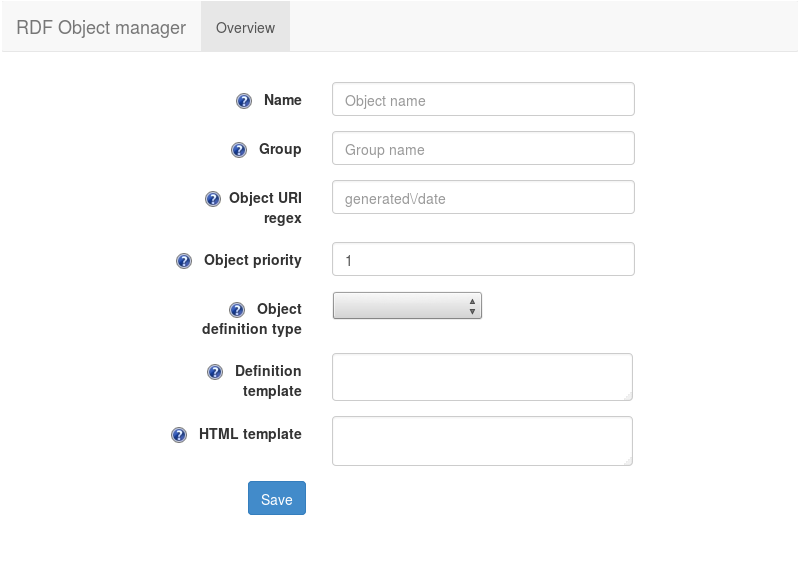
\includegraphics[width=\textwidth]{web_create}
 	\caption[Formulář pro založení a editaci definice]{Formulář pro založení a editaci definice}\label{web_create}		
  \end{figure}
    
    \subsection{Editace definic}
    Po kliknutí na tlačítko \uv{Edit} v přehledu definic je uživatel přesměrován na informace o dané definici.
    Tyto informace jsou přístupné v editovatelném formuláři. Tento formulář je strukturou totožný s 
    formulářem pro tvorbu nových definic.
    
    \subsection{Mazání definic}
    Uživatel může smazat konkrétní definici přes webovou aplikaci kliknutím na tlačítka \uv{Delete} a následním potvrzením.
    Smazanou definici již nejde žádným způsobem znovu obnovit.    
    
    \section{API}
    Administrace definic je také možná přes API. API podporuje všechny operace, které jsou popsány v kapitole \ref{web_app}. Struktura API včetně dotazů je
    popsána v návrhu v kapitole API \ref{api}.
    
    \section{Typy definic}\label{def_types}
    U každé následující definice jsou uvedeny příklady pro stejný typ objektu - logovací systém, který je také
    dostupný v příloze v ukázkových definicích. Jedná se o objekt logované informace nastavený pro URL adresu, která na konci obsahuje mezi lomítky
    hodnoty atributů pro ID logu, datum, zprávu a název třídy. 
    
    
    \begin{itemize}
          
    \item \textbf{RDF serializace}   
    
     Tento typ se dělí na definice dle konkrétních serializací - Turtle, N-Triples, RDF/XML a JSON-LD. Uživatel do šablony RDF entity dosadí
     již serializovaná data a na místech, kam se mají dosadit parametry z URL adresy, vytvoří placeholdery.
     Následující příklad šablony je typu Turtle:
     
     \begin{lstlisting}[float=htb,caption={Šablona RDF entity v Turtle formátu},label=list:spage]
@base <[@0, "^([^/]*\/[^/]*\/[^/]*\/[^/]*\/[^/]*)\/"]> .
@prefix rlog: 
<http://persistence.unileipzig.org/nlp2rdf/ontologies/rlog#>.
@prefix xsd: <http://www.w3.org/2001/XMLSchema#> .

<#[@6]> # log id 
	a rlog:Entry ;
  	rlog:level rlog:WARN ;
	rlog:date "[@7]T[@8]Z"^^xsd:dateTime ;
	rlog:className "[@9]";
	rlog:message "[@10]".
\end{lstlisting}
 
    \item \textbf{SPARQL Construct}
    
      Šablonou pro tento typ je SPARQL Construct dotaz, kde se jednotlivé parametry mohou například vytvářet pomocí funkce \textit{BIND()}.
      Tento typ definice díky jazyku 
      SPARQL doplňuje RDF serializace o další funkcionality tohoto dotazovacího jazyka.
      Příklad stejného objektu pro SPARQL dotaz:
      
      
           \begin{lstlisting}[float=htb,caption={Šablona SPARQL dotazu},label=list:spage]
PREFIX rlog:  
<http://persistence.unileipzig.org/nlp2rdf/ontologies/rlog#>
PREFIX xsd:   <http://www.w3.org/2001/XMLSchema#>
CONSTRUCT { 
?res a rlog:Entry ;
  	rlog:level rlog:WARN ;
	rlog:date "[@7]T[@8]Z"^^xsd:dateTime ;
	rlog:className "[@9]";
	rlog:message "[@10]".
  }
WHERE {
    BIND (URI('[@0, 
    "^([^/]*\/[^/]*\/[^/]*\/[^/]*\/[^/]*)\/"]#[@6]')
    AS ?res) }
\end{lstlisting}
      
      
    \item \textbf{SPARQL Endpoint}
    
      Tento typ je rozšířením typu SPARQL Construct. Dotaz je spouštěn vzdáleně na SPARQL endpointu, přes který je možné přistupovat k datasetům které jsou
      na endpointu dostupné. Tento typ podporuje dva typy dotazů - Construct a Describe a narozdíl od předchozího typu může obsahovat komplikovanější
      dotazy právě nad zmíněnými datasety.
      
      
    \item \textbf{Proxy}
    
      Uživatel může nakonfigurovat přeposílání požadavků na jiný server, který poskytuje také data v RDF serializacích. Jedná se o případy, kdy uživateli
      nestačí výše zmíněné typy a potřebuje nějaký sofistikovanější generátor pro konkrétní objekt. Server tedy pouze přeposílá požadavek a výsledná
      data poté serializuje dle požadavku klienta.
    
    \end{itemize}
    
    \section{Struktura šablony}\label{template_system}
    Strukturou šablony se rozumí text, který uživatel vyplní jako atribut \uv{šablona definice} nebo \uv{HTML šablona}. Do šablon jsou při přístupu klienta 
    doplněny informace z URL adresy a následně je za použití této šablony vygenerována výsledná HTML stránka nebo RDF entita.
    Struktura šablon je popsána v kapitole Šablonovací systém \ref{template_system}.
    
    
    \section{Vygenerování RDF entity na žádost klienta}\label{obj_access}
    Pro vygenerování RDF entity klient přistupuje na URL adresu ve formátu \texttt{http://example.com/data/?group=<group>\&url=<url>}, kde:
    \begin{itemize}
     \item \texttt{example.com} označuje adresu serveru
     \item \texttt{<group>} označuje skupinu, ve které se nachází požadovaná definice. Jedná se o nepovinný parametr, ale je doporučeno využívat ho při 
     každém požadavku. Vyhledávání konkrétní definice je s tímto parametrem rychlejší a tedy i klientovi je rychleji poskytnuta výsledná vygenerovaná entita.
     Jedná se o parametr \uv{skupina}, který uživatel zadává při tvorbě definice objektu, více je uvedeno v kapitole Definice objektů \ref{obj_def}.
     \item Parametr \texttt{<url>} identifikuje konkrétní definici objektu a je zároveň identifikátorem výsledné vygenerované RDF entity (IRI).
     Definice objektů obsahuje parametr \uv{regex} - regulární výraz, který uživatel nastavuje tak, aby mu odpovídaly URL adresy, které mají identifikovat
     konkrétní definici a entitu. Tento regulární výraz je popsán v kapitole \ref{def_create}
    \end{itemize}
    
    \subsection{Příklad definice a výsledné RDF entity}
    Pro shrnutí informací o generování a definic objektů bude sloužit příklad definice objektu \texttt{loggerTurtle}, který je dostupný v příloze
    ve složce ukázkových objektů \texttt{objects}, jedná se o soubor \texttt{logger\_turtle.ttl}.
    
    \subsubsection{Definice objektu} \label{example_def}
    Objekt \texttt{loggerTurtle} je definován těmito parametry:
    \begin{itemize}
     \item \textbf{název}: loggerTurtle
     \item \textbf{skupina}: dynrdf
     \item \textbf{regulární výraz}: \texttt{loggerTurtle}
     \item \textbf{priorita}: 1
     \item \textbf{typ definice}: TURTLE
     \item \textbf{šablona definice}: šablona definice je uvedena v kódu \ref{list:turtle}
          \begin{lstlisting}[float=htb,caption={Šablona RDF entity v Turtle formátu pro objekt loggerTurtle},label={list:turtle}]
@base <[@0, "^([^/]*\/[^/]*\/[^/]*\/[^/]*\/[^/]*)\/"]> .
@prefix rlog: 
<http://persistence.unileipzig.org/nlp2rdf/ontologies/rlog#>.
@prefix xsd: <http://www.w3.org/2001/XMLSchema#> .

<#[@6]> # log id 
	a rlog:Entry ;
  	rlog:level rlog:WARN ;
	rlog:date "[@7]T[@8]Z"^^xsd:dateTime ;
	rlog:className "[@9]";
	rlog:message "[@10]".
\end{lstlisting}
     \item \textbf{HTML šablona}: HTML šablona je uvedena v kódu \ref{list:html}
               \begin{lstlisting}[float=htb,caption={HTML šablona pro objekt loggerTurtle},label={list:html}]
<!doctype html>

<html lang="en">
  <head>
    <meta charset="utf-8">
    <title>Logger</title>
    <meta name="description" content="Dynrdf logger example">
  </head>

  <body>
    Log record: [@10] <br />
    Log ID: #[@6] <br />
    Level: Warn <br />
    Time: [@7] [@8] <br />
    Class name: [@9]
  </body>
</html>
\end{lstlisting}
    \end{itemize}
    
    Regulární výraz \texttt{loggerTurtle} a struktura šablon předepisují očekávanou strukturu URL adresy. Tou může být URL adresa  \\
    \texttt{http://example.com/data/?group=<group>\&url=<url>}, kde parametry \\ \texttt{group} a \texttt{url} obsahují hodnoty:
    \begin{itemize}
     \item \texttt{<group>}: dynrdf
     \item \texttt{<url>}: \texttt{http://logservice.com/data/loggerTurtle/42/2016-05-01/\\10:00:23/org.dynrdf.Request/some exception msg}
    \end{itemize}

    V této URL adrese parametr \texttt{group} odpovídá parametru definice (\texttt{dynrdf}) a URL adresa v parametru \texttt{url} odpovídá regulárnímu výrazu
    \texttt{loggerTurtle}, protože je přímo v URL uveden text \texttt{../loggerTurtle/..}. Vztah mezi URL adresou a regulárním výrazem je možné
    ověřit si online na adrese \url{http://regexr.com/3ddne}.
    
    URL adresa se v šablonovacím systému dělí na následující atributy mezi lomítky, které může uživatel použít v šablonách:
    \begin{itemize}
     \item \textbf{@0}: celá URL adresa
     \item \textbf{@1}: http:
     \item \textbf{@2}: prázdný řetězec (mezi //)
     \item \textbf{@3}: logservice.com
     \item \textbf{@4}: data
     \item \textbf{@5}: loggerTurtle
     \item \textbf{@6}: 42
     \item \textbf{@7}: 2016-05-01
     \item \textbf{@8}: 10:00:23
     \item \textbf{@9}: org.dynrdf.Request
     \item \textbf{@10}: some exception msg
    \end{itemize}
    Pokud je v šabloně uvedeno záporné číslo parametru, nebo URL adresa po zpracování neobsahuje dostatečný počet parametrů, je uživateli vrácena
    odpověď s kódem \texttt{400 - Bad Request}. Pokud by v tomto příkladě URL adresa neobsahovala poslední parametr (zprávu výjimky \uv{some exception msg}, nebo jinou zprávu),
    parametr \texttt{@10} by tedy nebyl nalezen a klientovi by byla odeslána odpověď se zmíněným kódem.

    
    \subsubsection{Výsledná RDF entita}
    Uživateli je přístupem na URL adrese uvedené v kapitole \ref{example_def} vygenerována výsledná entita. Typ serializace si vždy určuje klient technikou
    Content Negotioation \cite{content_negotiation}. V tomto příkladě je uveden výsledek ve formátu Turtle v kódu \ref{list:example_entity_turtle}
                   \begin{lstlisting}[float=htb,caption={Výsledná entita ve formátu Turtle pro příklad objektu loggerTurtle},label={list:example_entity_turtle}]
@prefix rlog:  
<http://persistence.uni-leipzig.org/nlp2rdf/ontologies/rlog/rlog.ttl> .
@prefix xsd:   <http://www.w3.org/2001/XMLSchema#> .

<http://logservice.com/data/loggerTurtle#42>
        a               rlog:Entry ;
        rlog:className  "org.dynrdf.Request" ;
        rlog:date       "2016-05-01T10:00:23Z"^^xsd:dateTime ;
        rlog:level      rlog:WARN ;
        rlog:message    "some exception msg" .
\end{lstlisting}

Přístupem klienta přes webový prohlížeč je vygenerována HTML stránka dle HTML šablony \label{list:html}. HTML šablona v tomto příkladu
obsahuje jen přehled atributů ekvivalentní RDF entity. Vzhled a obsah výsledné stránky si definuje každý uživatel při tvorbě definic sám.
Tato stránka je zobrazena na obrázku \ref{example_html_output}.
    \begin{figure}\centering
 	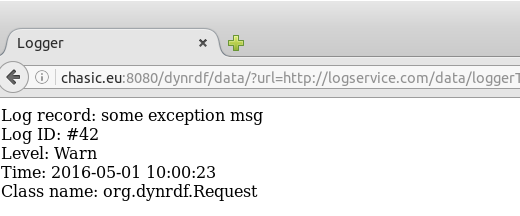
\includegraphics[width=\textwidth]{example_html_output}
 	\caption[Vygenerovaná HTML stránka pro příklad loggerTurtle]{Vygenerovaná HTML stránka pro příklad loggerTurtle}\label{example_html_output}		
  \end{figure}


    
  \section{Instalace serveru}
  Instalaci serveru je možné provést s již vytvořeným webovým archivem, který je k dispozici v příloze k práci (soubor \texttt{dynrdf.war}), nebo ze zdrojových kódů serveru,
  které jsou k této práci také přiloženy a které jsou také dostupné online v repozitáři \url{https://github.com/Chasic/dynrdf}.
  
  \subsection{Systémové požadavky}
  \begin{itemize}
   \item Webový server pro webové aplikace v Javě Tomcat \cite{tomcat_web} nebo Glassfish \cite{glassfish}
   \item Java 8 \cite{java8}
   \item Maven \cite{maven}
  \end{itemize}
    
  \subsection{Instalace přes webový archiv}\label{war_install}
  Instalace serveru přes přiložený webový archiv je nejjednodušší variantou. Pro správný chod celého serveru je potřeba před nasazením nastavit konfiguraci serveru.
  Celá instalace má následující kroky:
  \begin{itemize}
   \item V souborovém systému založte adresář pro definice objektů a zajistěte práva pro čtení a zápis pro webový server pod kterým aplikace běží
   \item Nakopírujte do tohoto adresáře ukázkové objekty z adresáře \texttt{objects}, který je k dispozici v příloze nebo online v repozitáři
   na adrese \url{https://github.com/Chasic/dynrdf/tree/master/objects}
   \item Otevřte přiložený soubor \texttt{dynrdf.war} v libovolném manažeru archivů
   \item V archivu otevřte soubor \texttt{/WEB-INF/classes/config.properties} dle obrázku \ref{config} a nastavte zde tyto parametry:
   
    \begin{itemize}
    \item \texttt{ObjectsPath}
    
    Cesta k adresáři s definicemi objektů
    \item \texttt{ObjectBaseUrl} 
    
    URL adresa na seznam objektů dostupný z API: \url{http://<host>/api/objects}, kde \texttt{<host>} je adresa serveru.
       
    \item \texttt{ObjectRDFS} 
    
    Cesta k RDF schématu, který definuje atributy definic, jako jsou typy definic, regulární výraz apod. Na této cestě by se měl vyskytovat obsah souboru 
    \texttt{dynrdf.rdfs.ttl}. Ten je v základu aplikace dostupný z kořene webové aplikace na adrese \url{http://<host>/dynrdf.rdfs.ttl}, kde \texttt{<host>} 
    je adresa serveru. Pro udržení konzistence v URL adresách je potřeba změnit tuto URL také v tomto souboru. Jedná se o řádek na začátku souboru:
    \\
      \texttt{ @prefix dynrdf: <http://dynrdf.com/dynrdf.rdfs.ttl\#>}
      \\	
      Na tomto řádku změnte URL ve špičatých závorkách na stejnou adresu, na které je tento soubor dostupný.
    
    
   \end{itemize}  
   Parametry \texttt{ObjectBaseUrl} a \texttt{ObjectRDFS} se používají při ukládání definic do Turtle formátu.
  

   \item V archivu otevřte soubor \texttt{/WEB-INF/classes/log4j.properties} a nastavte zde parametr \texttt{log4j.appender.file.File} na cestu,
   kam chcete ukládat logy.
   Můžeté také změnit styl logování, případně změnit i typ logování z \texttt{DEBUG} na jiný typ prostředí.
   \item Uložte upravený webový archiv
   \item Nahrajte soubor \texttt{dynrdf.war} na aplikační server. Na serveru Tomcat pomocí formuláře pro nahrání na obrázku \ref{tomcat_deploy}.
  \end{itemize}

      \begin{figure}\centering
 	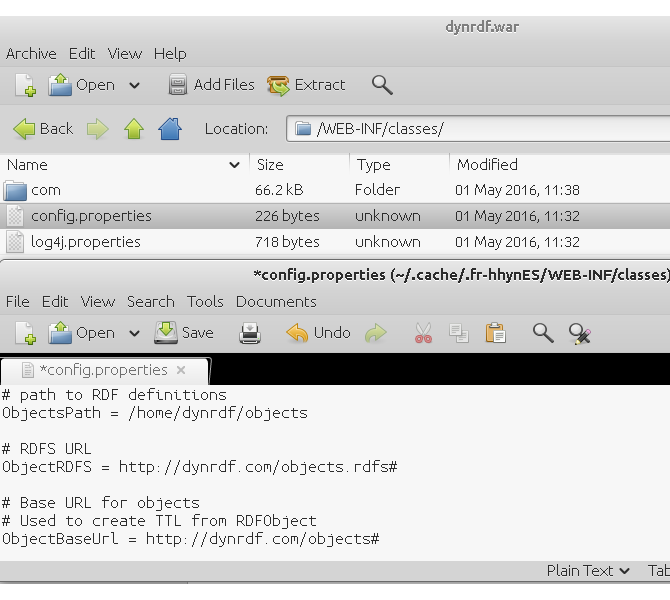
\includegraphics[width=\textwidth]{config}
 	\caption[Nastavení parametrů v konfiguračním souboru]{Nastavení parametrů v konfiguračním souboru}\label{config}		
  \end{figure}
  
        \begin{figure}\centering
 	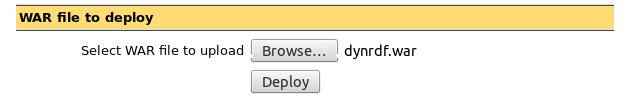
\includegraphics[width=\textwidth]{tomcat_deploy}
 	\caption[Nahrání webového archivu na server Tomcat]{Nahrání webového archivu na server Tomcat (adresa /manager/html) - vyberte war soubor z adresáře a klikněte na deploy}\label{tomcat_deploy}		
  \end{figure}
  

  
  \subsection{Instalace ze zdrojových kódů}
  Pro instalaci ze zdrojových kódu je potřba mít nainstalovaný program Maven.
  Instalace má tyto kroky:
   \begin{itemize}
   \item Nastavte parametry v konfiguračních souborech podobně jako při instalaci z připraveného war souboru. Konfigurační soubory se
   nacházejí ve složce \texttt{src/main/resources}.
   \item Vytvořte ze zdrojových kódů webový archiv pomocí příkazu \texttt{mvn package} v kořenu zdrojových kódu (tam kde je uložen soubor \texttt{pom.xml}).
   \item Webový archiv \texttt{dynrdf.war}, který najdete ve složce \texttt{target}, která se po provedení příkazu vytvořila, nahrajte na aplikační server stejně jako 
   v případě instalace serveru z war souboru \ref{war_install}.

  \end{itemize}
  
  \section{Nastavení serveru pro původ dat}
  Struktura URL adresy tak, jak je popsána v kapitole \ref{sec:identifikace}, podporuje možnosti pro nastavení webových serverů tak, aby 
  vůči klientům vystupovaly jako servery, na kterých jsou data uložena, ikdyž jsou generované touto aplikací na jiném serveru (na jiné URL adrese). Tímto chováním je docíleno konzistence
  mezi URL adresou, na které je RDF entita dostupná a IRI této entity ve vygenerovaném souboru.
  
  Pro demonstraci slouží následující příklad. Ten popisuje chování pro už dříve zmiňovanou definici RDF entity logovací služby. Předpokládejme, že webový server
  pro dynamické generování je v tomto příkladu dostupný na adrese \url{http://dynrdf.com} a server pro původ dat je dostupný na adrese\\ 
  \url{http://logservice.com}. 
  
  Ze šablony pro RDF entitu \ref{list:example_template} je důležitý řádek s identifikátorem entity, 
  konkrétně jde o placeholder v \texttt{<[@0]>}. Za placeholder \texttt{[@0]} se dosazuje celá URL adresa. Za URL adresu, kde má být přístupná požadovaná RDF entita
  nadále považujme URL \url{http://logservice.com/data/loggerTurtle/42/2016-05-01/10:00:23/org.dynrdf.Request/msg}. 
  

\begin{lstlisting}[float=htb,caption={Šablona RDF entity v Turtle formátu},label=list:example_template]
@prefix rlog: 
<http://persistence.unileipzig.org/nlp2rdf/ontologies/rlog#>.
@prefix xsd: <http://www.w3.org/2001/XMLSchema#> .

<[@0]> 
	a rlog:Entry ;
  	rlog:level rlog:WARN ;
	rlog:date "[@7]T[@8]Z"^^xsd:dateTime ;
	rlog:className "[@9]";
	rlog:message "[@10]".
\end{lstlisting}
  \newpage
  K nekonzistenci mezi URL adresou, kde je RDF entita dostupná a její IRI dochází v případě, kdy klient přistoupí přímo na URL adresu 
  \url{http://dynrdf.com/data/?url=http://logservice.com/data/loggerTurtle/4111/2016-05-01/10:00:23/org.dynrdf.Request/msg}.
  V tomto případě je výsledná RDF entita vygenerována na dané URL, ale její IRI je rovno hodnotě GET parametru \texttt{url}.
  
  Toto chování lze opravit pomocí nastavení webového serveru, kde je aplikace \url{http://logservice.com} spuštěna.
  Toto nastavení musí zařídit přeposílání požadavků na RDF entitu přes proxy na server pro generování. 
  Například ve webovém serveru Apache \cite{apache_httpd} se dá toto přeposílání nastavit
  s použitím modulu \texttt{mod\_rewrite} \cite{mod_rewrite}, jak je uvedeno v ukázce konfigurace \ref{list:apache_config}.
  
  Klíčový je zde řádek s \texttt{RewriteRule}, který ve volném překladu znamená: \uv{Pro všechny požadavky na data přesměruj tyto požadavky na adresu 
  serveru pro dynamické generování. Jako \texttt{url} parametr nastav adresu požadavku.}.  Parametrem \texttt{[P]} je docíleno toho, že je použit modul 
  \texttt{mod\_proxy} \cite{mod_proxy} a nedochází tedy k přímému přesměrování, ale klientovi se jeví výsledná data tak, že pocházejí z dané URL adresy.
  
  Pokud tedy klient přistoupí na URL adresu \url{http://logservice.com/data/loggerTurtle/42/2016-05-01/10:00:23/org.dynrdf.Request/msg},\\ získá výslednou RDF entitu
  a URL adresa i IRI entity se budou shodovat. K přesměrování požadavku na server pro vygenerování entity proběhlo na pozadí a klientovi se výsledná data jeví tak,
  že pochází se serveru\\ \url{http://logservice.com}.
  
  \begin{lstlisting}[float=htb,caption={Část konfigurace webového serveru Apache sloužící k přeposílání požadavků přes proxy},label=list:apache_config]
RewriteEngine  on
RewriteRule    /data/(.*)  
  http://dynrdf.com/data/?url=http://%{REMOTE_HOST}%{SCRIPT_FILENAME}  
  [P]

\end{lstlisting}
  
  
\begin{conclusion}
Cílem této práce bylo navrhnout, implementovat a otestovat webový server pro poskytování dynamicky generovaných objektů v RDF formátech.
Serveru byly určeny požadavky zadáním této práce a také dalšími v průběhu tvorby této práce. Dalšími požadavky se zabývala převážně analytická část.

Všechny tyto požadavky a cíle byly splněny.
Návrhu předcházela analýza účelu aplikace a podobných řešení. Závěrem této analýzy bylo, že neexistuje žádný server, který by poskytoval funkce
implementovaného serveru. To dává této práci šanci být využívanou ve velkém měřítku.

Na základě analýzy byl proveden návrh celého systému a následně jeho implementace. Bylo použito několik pokročilých technologií jak z oboru Linked Data,
tak i z pohledu implementace.

Testování proběhlo na několika úrovních. Základem byly unit testy netriviálních metod tříd, na které navázaly komplexnější testy celé aplikace.
Server byl také otestován na výkon.


Mně osobně přinesla tato práce mnoho nových zkušeností a znalostí. Jedná se převážně o obor Linked Data, který mne velice zaujal a plánuji se mu i dále věnovat.
Z pohledu implementace se jednalo o zatím největší aplikaci v Javě, kterou jsem programoval. Vyzkoušel jsem si práci s velkým množstvím kvalitních knihoven,
které se ve světě velmi často používají. Z pohledu testování jsem si osvojil nové techniky testování aplikací v Javě, především těch webových. Také jsem se poprvé
věnoval testování výkonu webové aplikace.
Ve vývoji této práce plánuji i nadále pokračovat.


S využitím této práce se počítá pro datasety otevřené datové infrastruktury opendata.cz.		

\end{conclusion}

\bibliographystyle{csn690}
\bibliography{mybibliographyfile}

\appendix

\chapter{Seznam použitých zkratek}
% \printglossaries
\begin{description}
	\item[RDF] Resource description framework
	\item[URI] Uniform Resource Identifier
	\item[IRI] Internationalized Resource Identifier
	\item[URL] Uniform Resource Locator
	\item[HTTP] Hypertext Transfer Protocol
	\item[WWW] World Wide Web
	\item[HTML] HyperText Markup Language
	\item[SPARQL] Protocol and RDF Query Language
	\item[API] Application program interface
	\item[CRUD] Create, read, update and delete
	\item[IP] Internet Protocol 
	\item[MVC] Model–view–controller
	\item[JSON] JavaScript Object Notation
	\item[VPS] Virtual private server
\end{description}



\chapter{Obsah přiloženého CD}
\begin{figure}[H]
	\dirtree{%
		.1 readme.txt\DTcomment{stručný popis obsahu CD}.
		.1 install.txt\DTcomment{instalační pokyny pro nasazení war souboru}.
		.1 dynrdf.war\DTcomment{war soubor pro deploy na server}.
		.1 objects\DTcomment{adresář s ukázkovými definicemi objektů}.
		.1 testObjects\DTcomment{adresář s definicemi objektů pro testování}.
		.1 img \DTcomment{adresář s obrázky}.
		.1 src.
		.2 impl\DTcomment{zdrojové kódy implementace}.
		.2 thesis\DTcomment{zdrojová forma práce ve formátu \LaTeX{}}.
		.1 text\DTcomment{text práce}.
		.2 thesis.pdf\DTcomment{text práce ve formátu PDF}.
	}
\end{figure}

\end{document}
